In this chapter, the control algorithms designed for the system are presented, along with their implementation and simulation in MATLAB. The primary objective is to evaluate the performance of different control strategies and analyze their effectiveness in achieving the desired system response. Simulations are then conducted to assess system stability, transient behavior, and robustness under varying conditions.

\section{Full State Feedback}
A full state feedback controller, also referred to as a pole placement controller which is shown in figure \ref{fig:stfb}, provides an optimal solution for achieving desired pole locations of a closed-loop system. This approach leverages the fact that all state variables are assumed to be known to the controller at all times and are available for feedback.

The state-space representation of the plant is utilized, where each state variable is fed back to the control input, u, through a gain matrix, K. This feedback gain matrix can be adjusted to achieve the desired closed-loop pole values.

\begin{figure}[H]
	\centering
	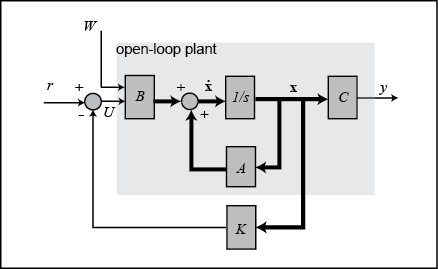
\includegraphics[width=0.4\textwidth]{stfb.png}
	\caption{Full state feedback block diagram. \cite{controltutorials}
	}
	\label{fig:stfb}
\end{figure}

Assuming no tracking $(r=0)$ and no external disturbance $(w=0)$, the system input is given by:

$u = -Kx$

$\dot{x} = Ax - BKx$

$\dot{x} = x(A - BK)$

\section{Linear Quadratic regulator}
\subsection{Overview}
LQR controller is a widely used type of state feedback control that offers a systematic method for determining the control gain, $K$. The LQR approach will be employed in the controller design for the active suspension system, as it is a classic and straightforward option for linear, time-invariant, multiple-input multiple-output (MIMO) systems. One of the key advantages of using an LQR controller is its ability to weight the factors affecting the performance index based on the desired outcome. For this project, the focus of the LQR approach will be on enhancing ride comfort and improving road-handling performance in the quarter-car model.

\newpage
The function of an LQR controller is to minimize the cost function, J, which is shown in the following equation:

\[
J = \frac{1}{2} \int_{0}^{t} (x^{T}Qx + u^{T}Ru) \, dt 
\]

$x^{T}$ = State vector. 

$u^{T}$ = Input vector.


\subsection{LQR Implementation}
The weighting matrices, Q and R, within the quadratic performance index significantly influence the LQR controller's behavior. These matrices allow for tuning the control system's priorities, such as emphasizing ride comfort or minimizing control effort. The optimal values for Q and R were determined through iterative simulations and tuning within the MATLAB environment. This process involved systematically adjusting the elements of Q and R and observing the resulting system response to determine the combination that best met the desired performance objectives.\\ 

The following figure\ref{fig:lqr-final} shows the model used to simulate the dynamics of the quarter car suspension system, based on the state space model represented in the previous chapter. 

        \begin{figure}[H]
	\centering
	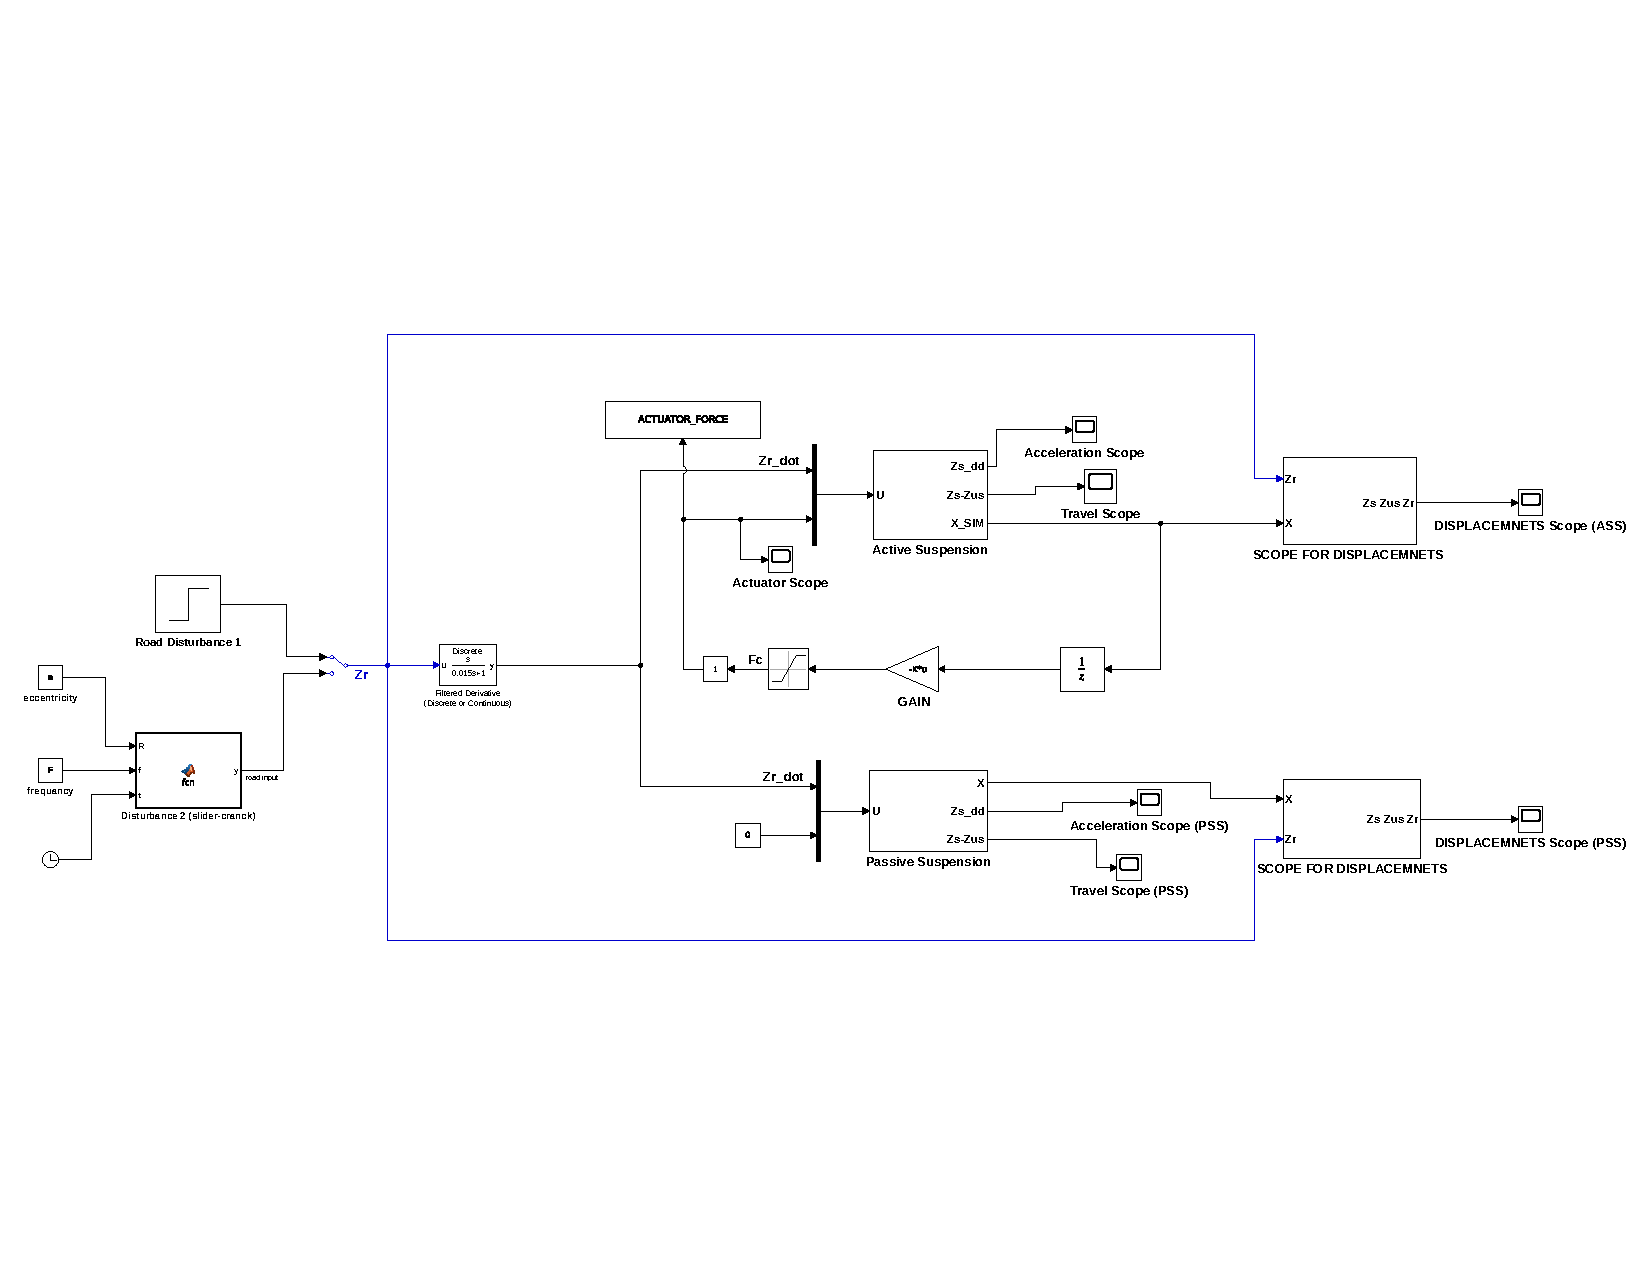
\includegraphics[trim=0cm 5cm 0cm 5cm, clip, width=1\linewidth]{figures/lqr-final.pdf}
	\caption{provides the block diagram model for the active suspension system}
	\label{fig:lqr-final}
\end{figure}


\section{LQR Simulation Results}
To evaluate the performance of the LQR controller we will compare between the passive suspension system and the active suspension sytem in case of two road excitation profiles, the first one will be a simple step input, the second one will be the profile of the slider crank mechanism, that we discussed in the previous chapter (section 3.3)

\newpage
\subsection{Step Response}
The following figure\ref{fig:step-sprungs} shows the effect of LQR on the system, it is a comparison between the passive and active response when excited by a step input of 60 mm amplitude.
 \begin{figure}[H]
	\centering
	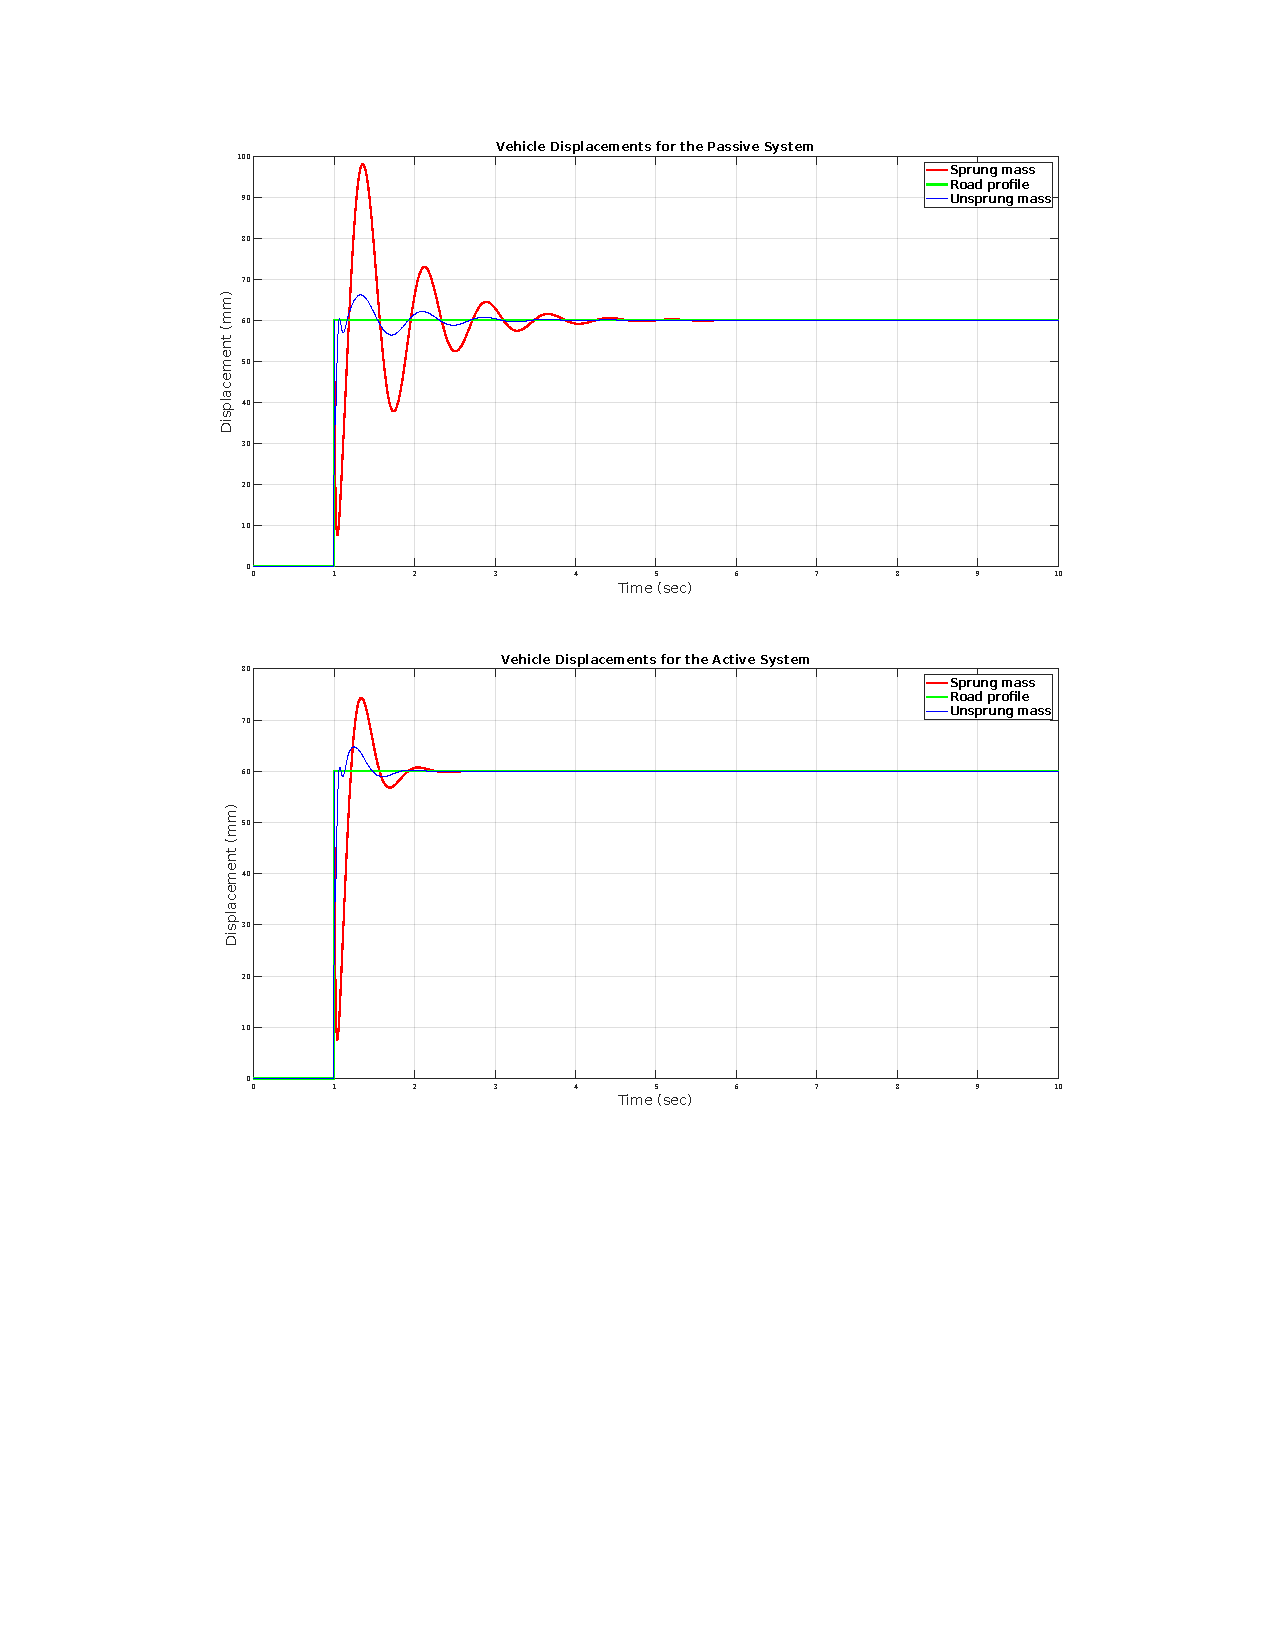
\includegraphics[trim=0cm 9cm 0cm 2cm, clip, width=1\linewidth]{figures/sprung-masses.pdf}
	\caption{Effect of the controller on Sprung and unsprung mass of the system}
	\label{fig:step-sprungs}
\end{figure}

\newpage
The following figures\ref{fig:all-step} compare between the performance of the system with LQR and without it to a step input: 
\begin{figure}[H]
	\centering
	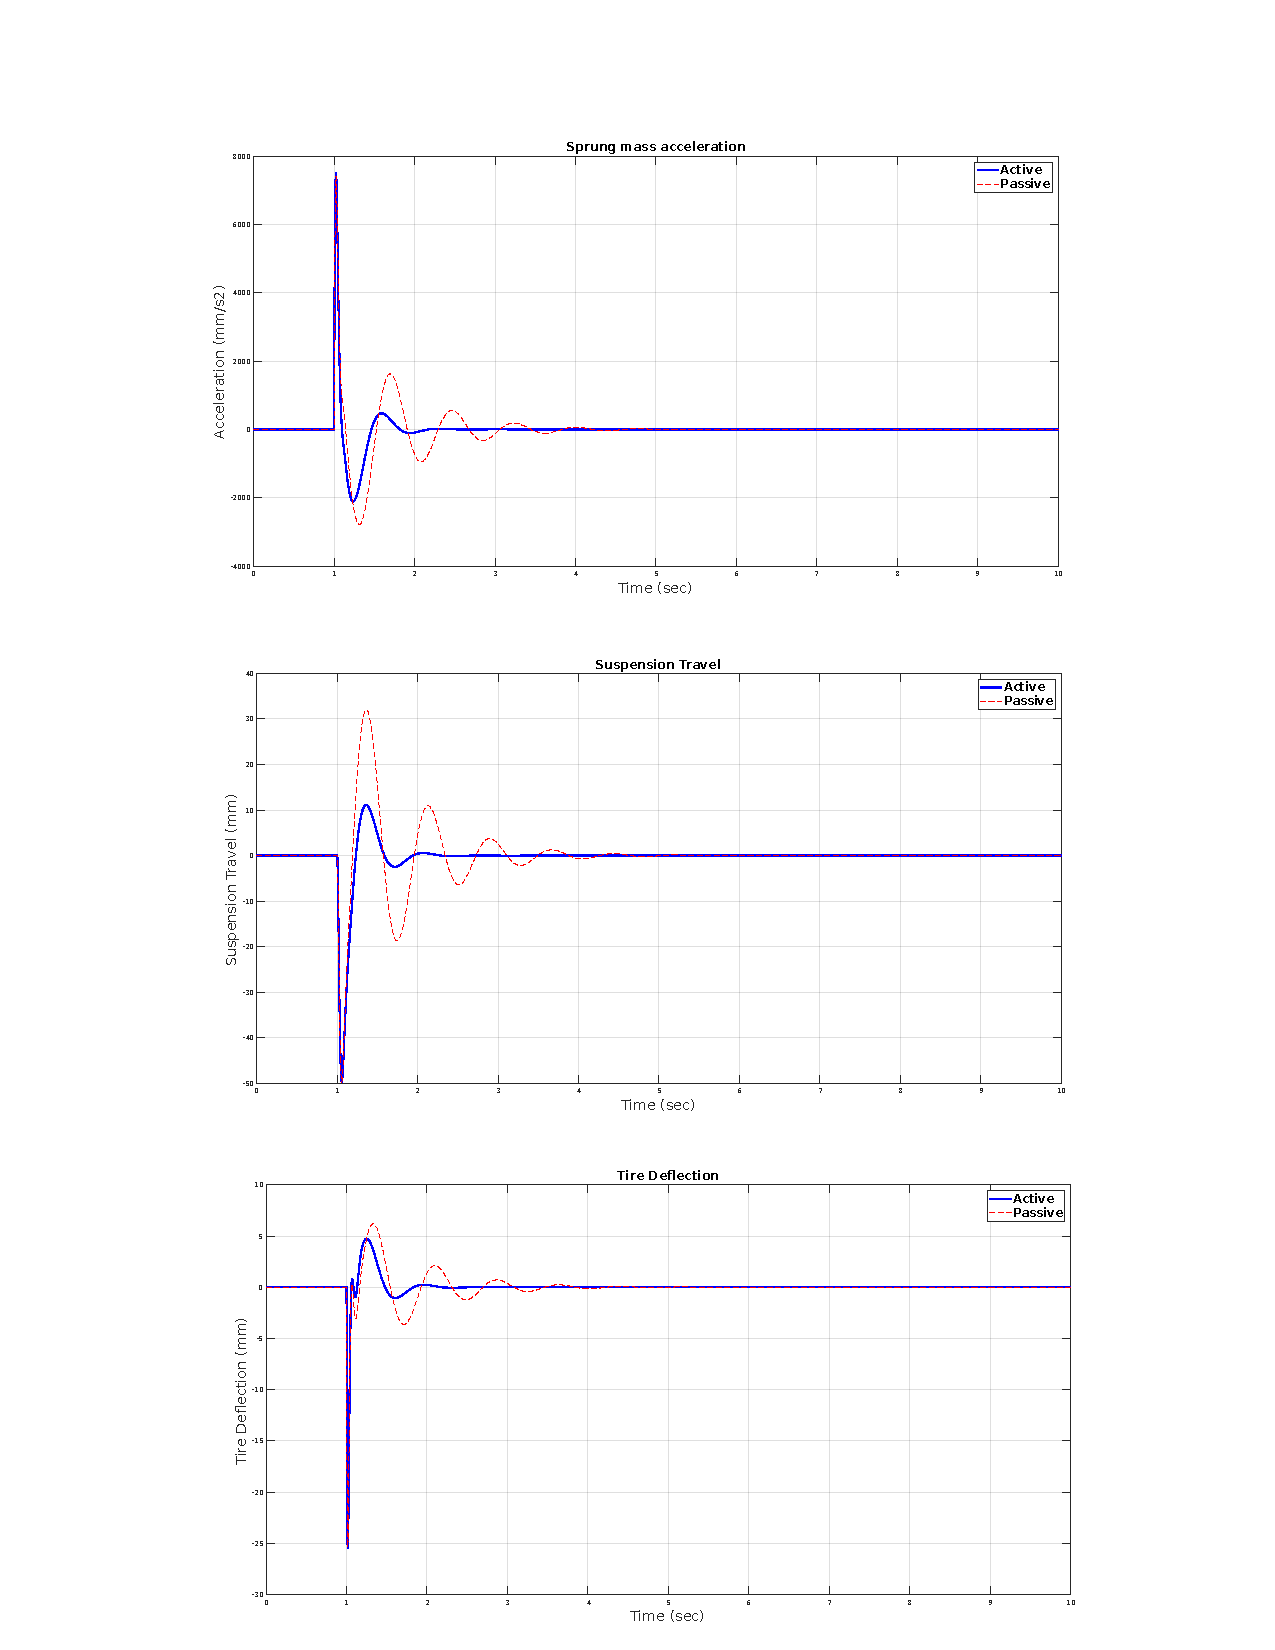
\includegraphics[trim=0cm 2cm 0cm 2cm, clip, width=1\linewidth]{figures/p-a-step.pdf}
	\caption{Effect of the controller}
	\label{fig:all-step}
\end{figure}

\newpage
\subsection{Road Profile Excitation}
This section shows the effect of the controller on the system against a more complicated road disturbance, which is the continuous excitation of the slider crank mechanism at a frequency of 0.3 HZ.

The following figures\ref{fig:road-sprungs} compare between the sprung and unsprung mass acceleration in both the passive and active systems:

 \begin{figure}[H]
	\centering
	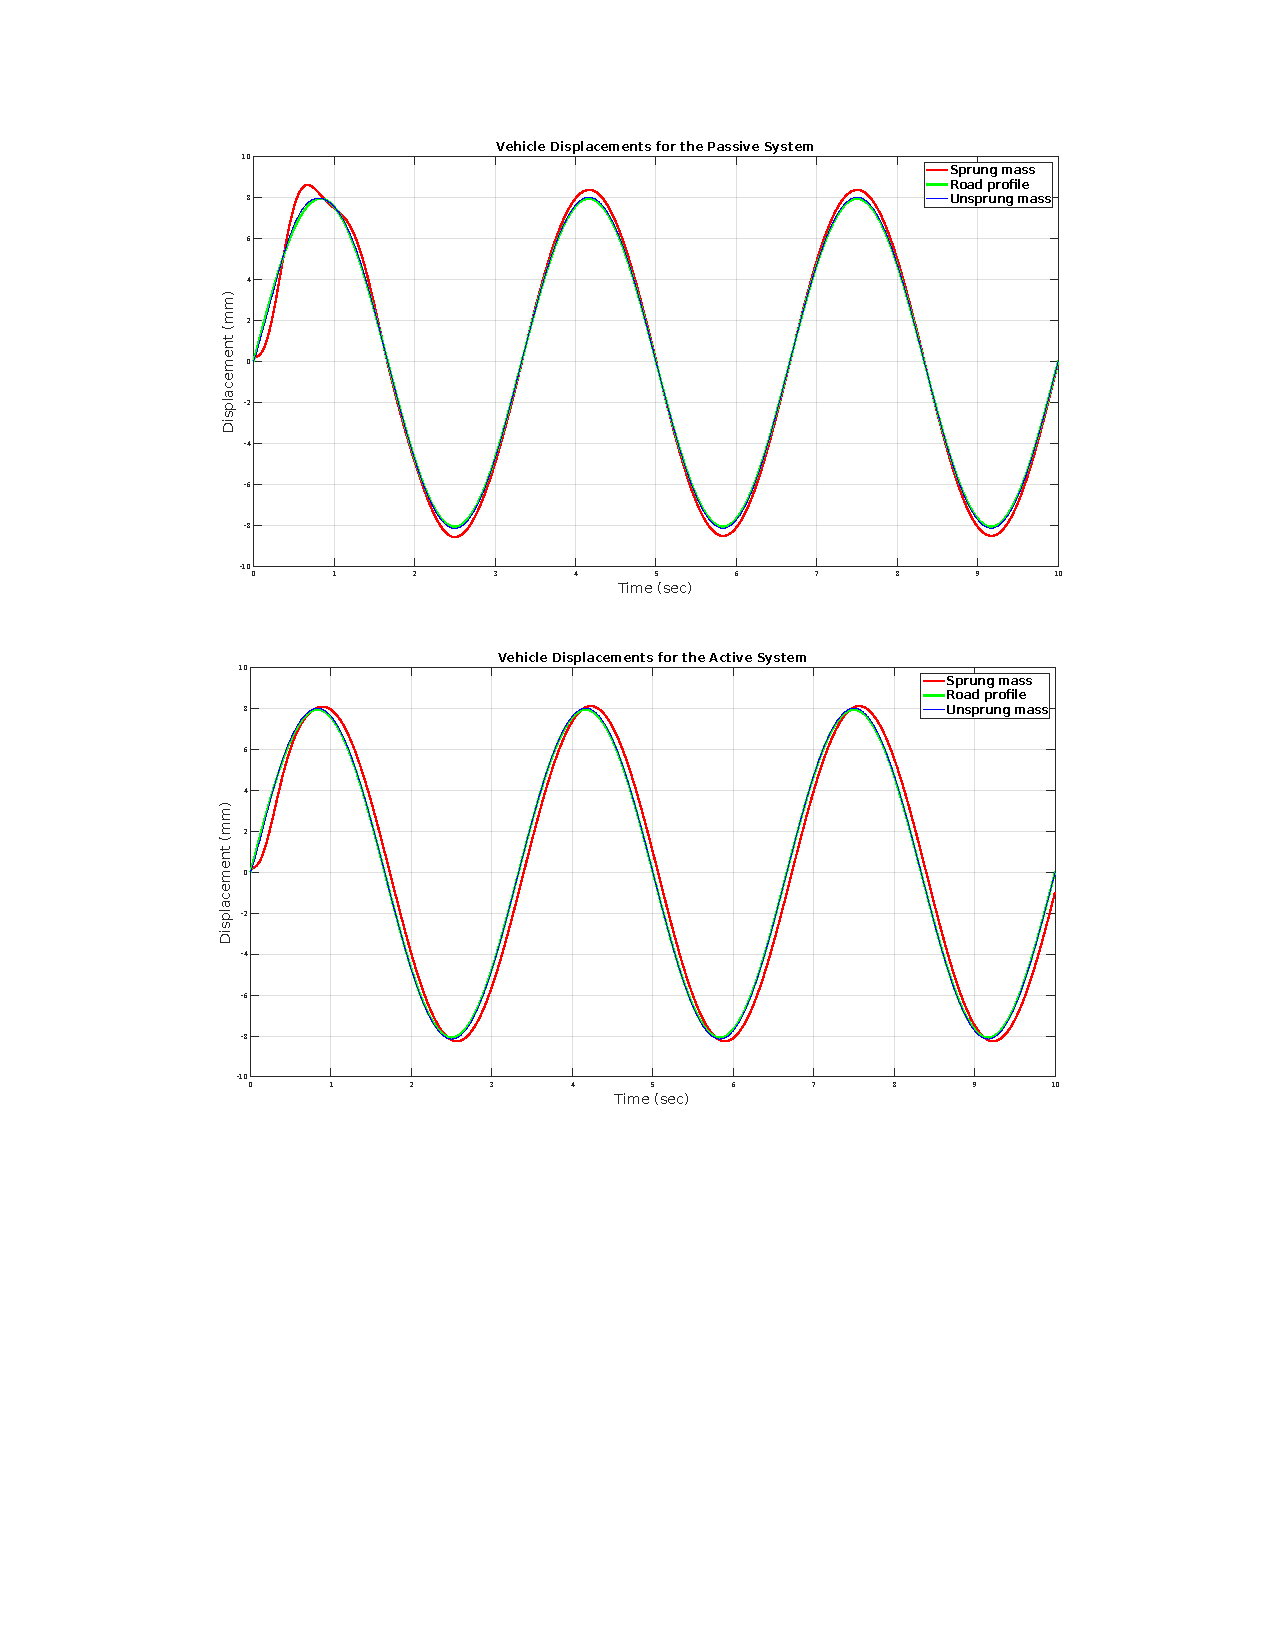
\includegraphics[trim=0cm 9cm 0cm 2cm, clip, width=1\linewidth]{figures/road-sprungs.pdf}
	\caption{Effect of the controller on Sprung and unsprung mass of the system}
	\label{fig:road-sprungs}
\end{figure}

\newpage
The following figures\ref{fig:all-road} compare between the performance of the system with LQR and without it, against the excitation of the road profile:
\begin{figure}[H]
	\centering
	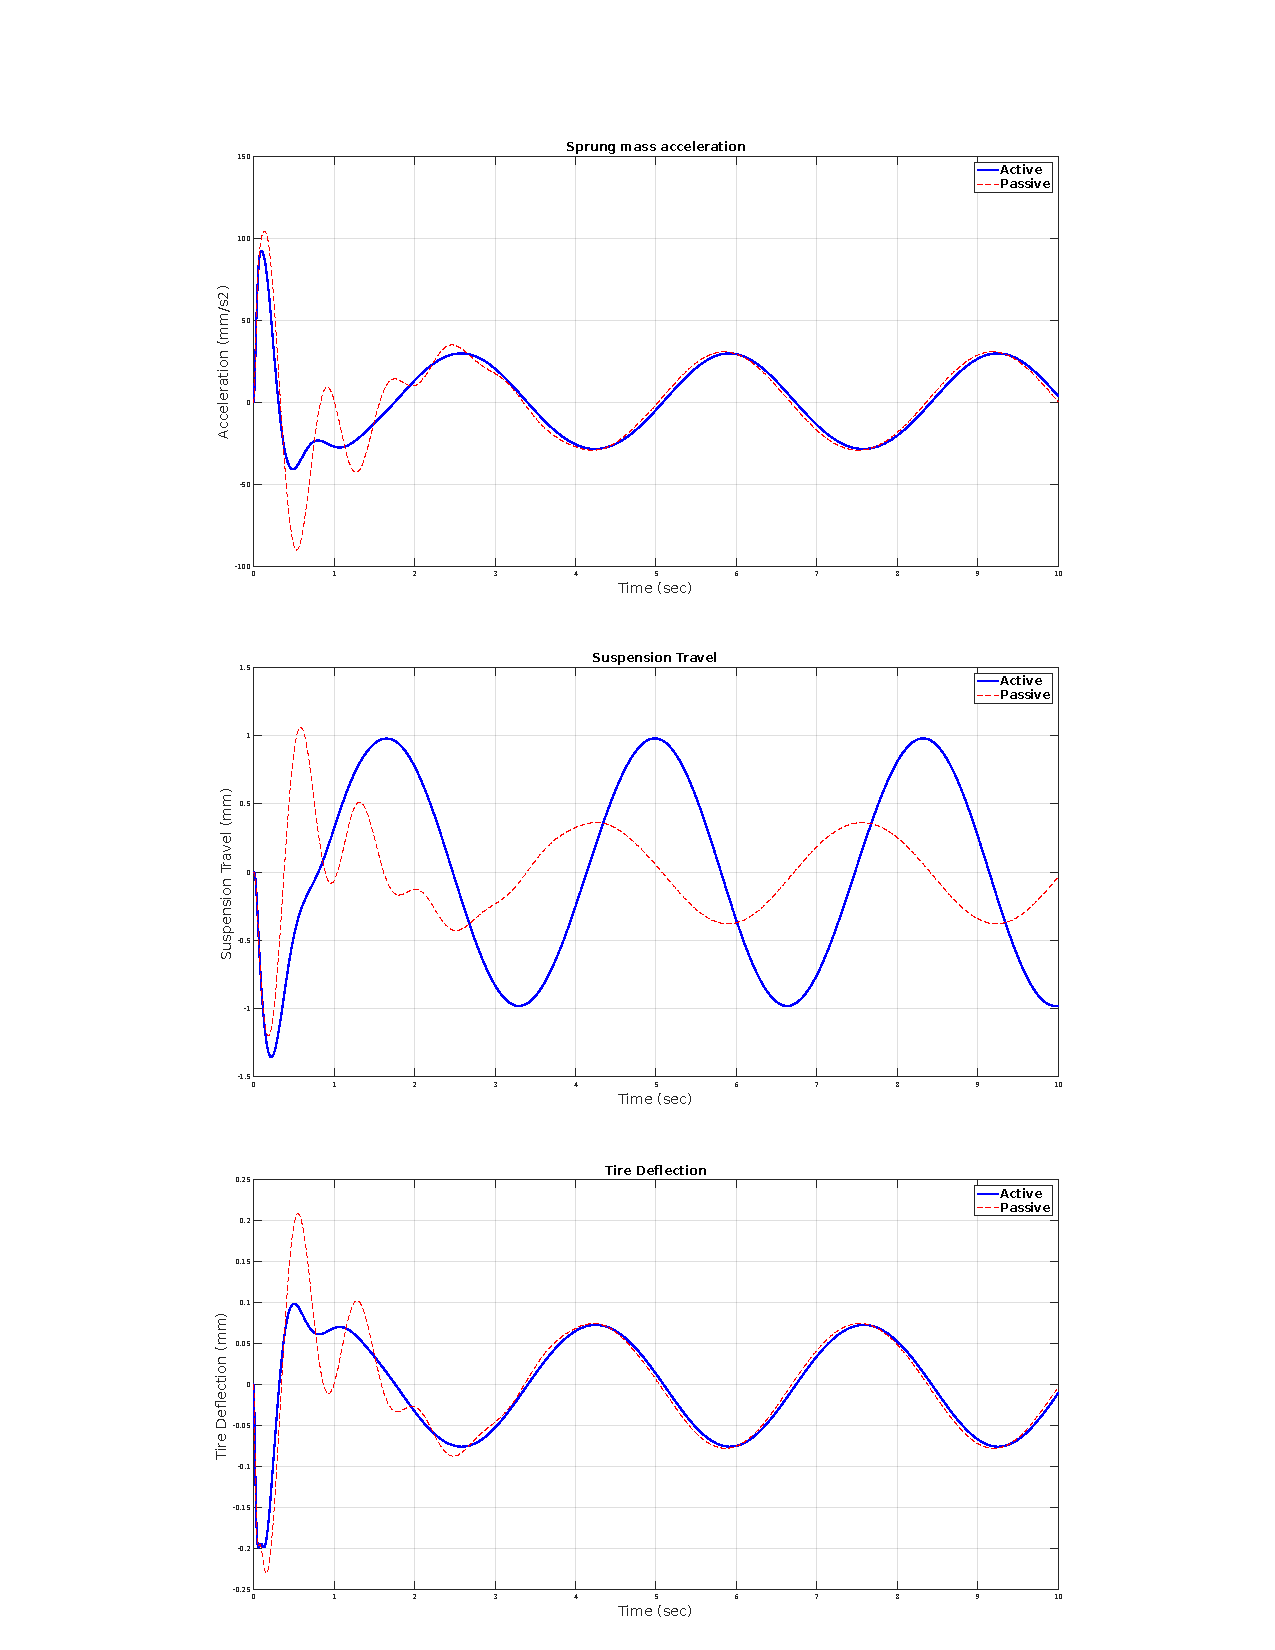
\includegraphics[trim=0cm 2cm 0cm 2cm, clip, width=1\linewidth]{figures/p-a-road.pdf}
	\caption{Effect of the controller}
	\label{fig:all-road}
\end{figure}

\newpage
\section{Sliding mode control}
\subsection{Overview}
Sliding Mode Control (SMC) is a nonlinear control technique featuring
remarkable properties of accuracy, robustness, and easy tuning and implementation. There are
two main advantages of sliding mode control. First is that the dynamic behavior of the system may
be tailored by the particular choice of the sliding function. Secondly, the closed loop response
becomes totally insensitive to some particular uncertainties. This principle extends to model
parameter uncertainties, disturbance and non-linearity that are bounded. From a practical point
of view (SMC) allows for controlling nonlinear processes subject to external disturbances and
model uncertainties
\subsection{Theory}
This is a type of non-linear control that provides a sporadic control signal in the process of altering dynamic characteristics of a system. The sliding mode control (SMC) is based on the principle of switching logic between different independent structural systems. The control strategy forces the system to slide along the normal behavioural lines. The control system is structured in such a way that paths always move towards a neighbouring region of the behavioural line with a different degree of control so that the ultimate path would not occur exclusively within one control. It will instead slide along the limits of the controlled structures while minimizing error, as indicated in \ref{fig:smc}. The SMC is, therefore, able to control both linear and non-linear systems. (1) The controller and (2) the sliding surface are the primary parameters of SMC.
\begin{figure}[H]
	\centering
	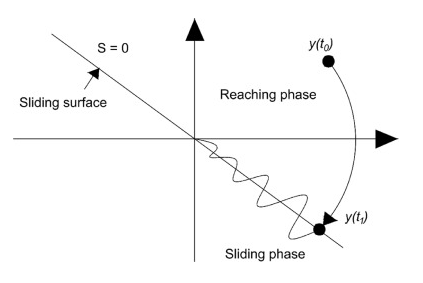
\includegraphics[width=0.4\textwidth]{SMC_theory.png}
	\caption{Representation of sliding surface and minimization of error. \cite{WANI2022103}
	}
	\label{fig:smc}
\end{figure}
\subsection{SMC implementation}
Using regulation mode to minimize system vibrations and improve ride comfort the first step is to define the sliding surface 
\subsubsection{Dfinning the sliding surface}
The sliding surface (or switching surface) is a key component of the SMC. It defines the condition under which the system behavior will enter a "sliding" mode. The sliding-mode surface can be described as:
\begin{equation}
	s = cZ_s+\dot{Z_s}
\end{equation}

\subsubsection{Design reaching law}
The reaching law ensures that the state of the system moves towards the sliding surface whatever its initial conditions. The reaching law is given by:
\begin{equation}
	h\left(s\left(x\right)\right) = -\eta sign\left(s\right)
\end{equation}
where $\eta$ is a positive constant that determines the speed of convergence to the sliding surface.

\subsubsection{Design the control law}
The sliding mode control law is designed to drive the system towards the sliding surface.
The derivative of s is given by:
\begin{equation}
	\dot{s} = c\dot{Z_s}+\ddot{Z_s}
	\label{equ:43}
\end{equation}
From mathematical model equation (\ref*{equ:ddzs}) the sprung mass acceleration is given by:
\begin{equation}
	\ddot{Z}_s = \frac{B_s\dot{Z}_{us}}{M_s} - \frac{B_s\dot{Z}_s}{M_s} - \frac{K_s(Z_s - Z_{us})}{M_s} + \frac{1}{M_s}F_c
\end{equation}
substitute in \ref{equ:43} :
\begin{equation}
	\dot{s} = c\dot{Z_s}-\frac{K_s}{M_s}Z_s + \frac{K_s}{M_s}Z_us + \frac{1}{M_s}F_c
\end{equation}
Let $\dot{s} = -\eta sign\left(s\right) $
\begin{equation}
	-\eta sign\left(s\right)= c\dot{Z_s}-\frac{K_s}{M_s}Z_s + \frac{K_s}{M_s}Z_us + \frac{1}{M_s}F_c
\end{equation}
Therefore, sliding-mode control input is given by :
\begin{equation}
	F_c= -cM_s\dot{Z_s}+K_sZ_s - K_sZ_us -\eta M_s sign\left(s\right)
\end{equation}
\subsubsection{Define boundary layer}
Using a saturation boundary layer instead of the sign function can effectively reduce the chattering effect. The idea is to apply the full gain when the system state is outside the boundary layer. However, once the system enters the boundary layer, the gain is made proportional to the distance from the boundary, effectively smoothing the control action. This modification ensures a continuous control signal within the boundary layer, mitigating chattering while maintaining robustness.
\begin{equation}
	\text{sat}(s, \phi) =
	\begin{cases} 
		1 & \text{if } s > \phi, \\
		\frac{s}{\phi} & \text{if } -\phi \leq s \leq \phi, \\
		-1 & \text{if } s < -\phi.
	\end{cases}
\end{equation}
After designing the control force to enhance the performance of the suspension system, the next step is to implement the Sliding Mode Controller (SMC) using MATLAB/Simulink.
\begin{figure}[H]
	\centering
	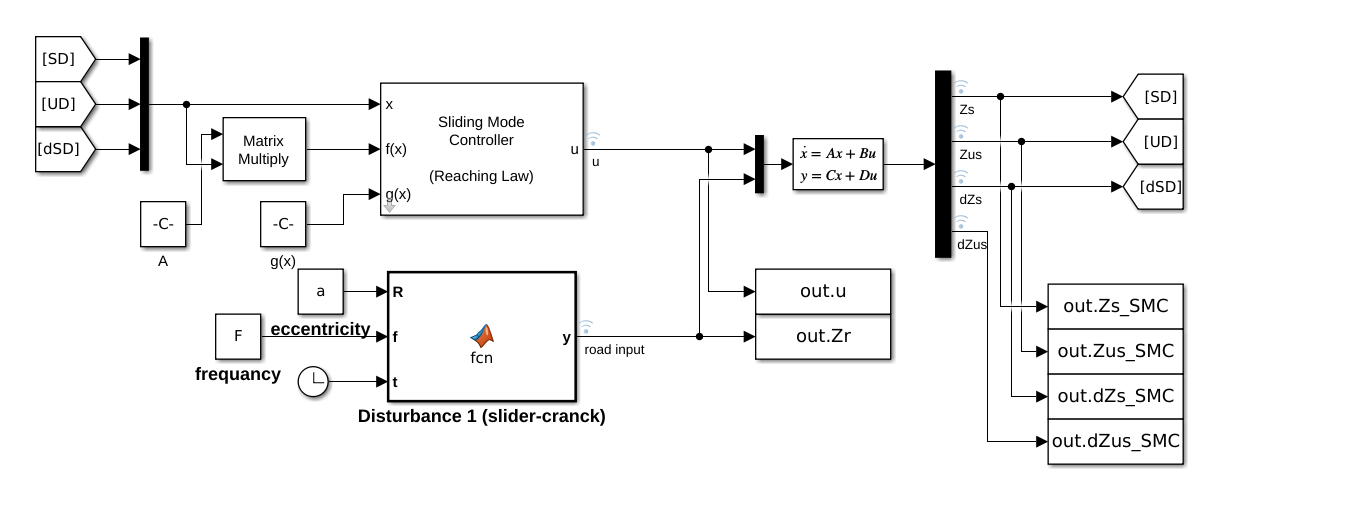
\includegraphics[width=1\textwidth]{SMC_simulink}
	\caption{SMC simulink model 
	}
	
\end{figure}
\section{SMC Simulation Results}
\begin{table}[h]
	\centering
	\caption{Simulation peak values of key indicators at 0.3 Hz,8 mm}
	\begin{tabular}{lccccc}
		
		\hline
		\textbf{} & \textbf{SD[mm]} & \textbf{UD[mm]}  & \textbf{ST[mm]}  & \textbf{DTD[mm]}  & \textbf{Fc[mm]}  \\
		\hline
		
		Passive & 9.07 & 8.15 & 1.05 & 0.25 & - \\
		SMC & 0.29& 8.09 & 7.97 &  0.178 & 55.72 \\
		
		
		\hline
		
	\end{tabular}
\end{table}

\begin{figure}[H]
	\centering
	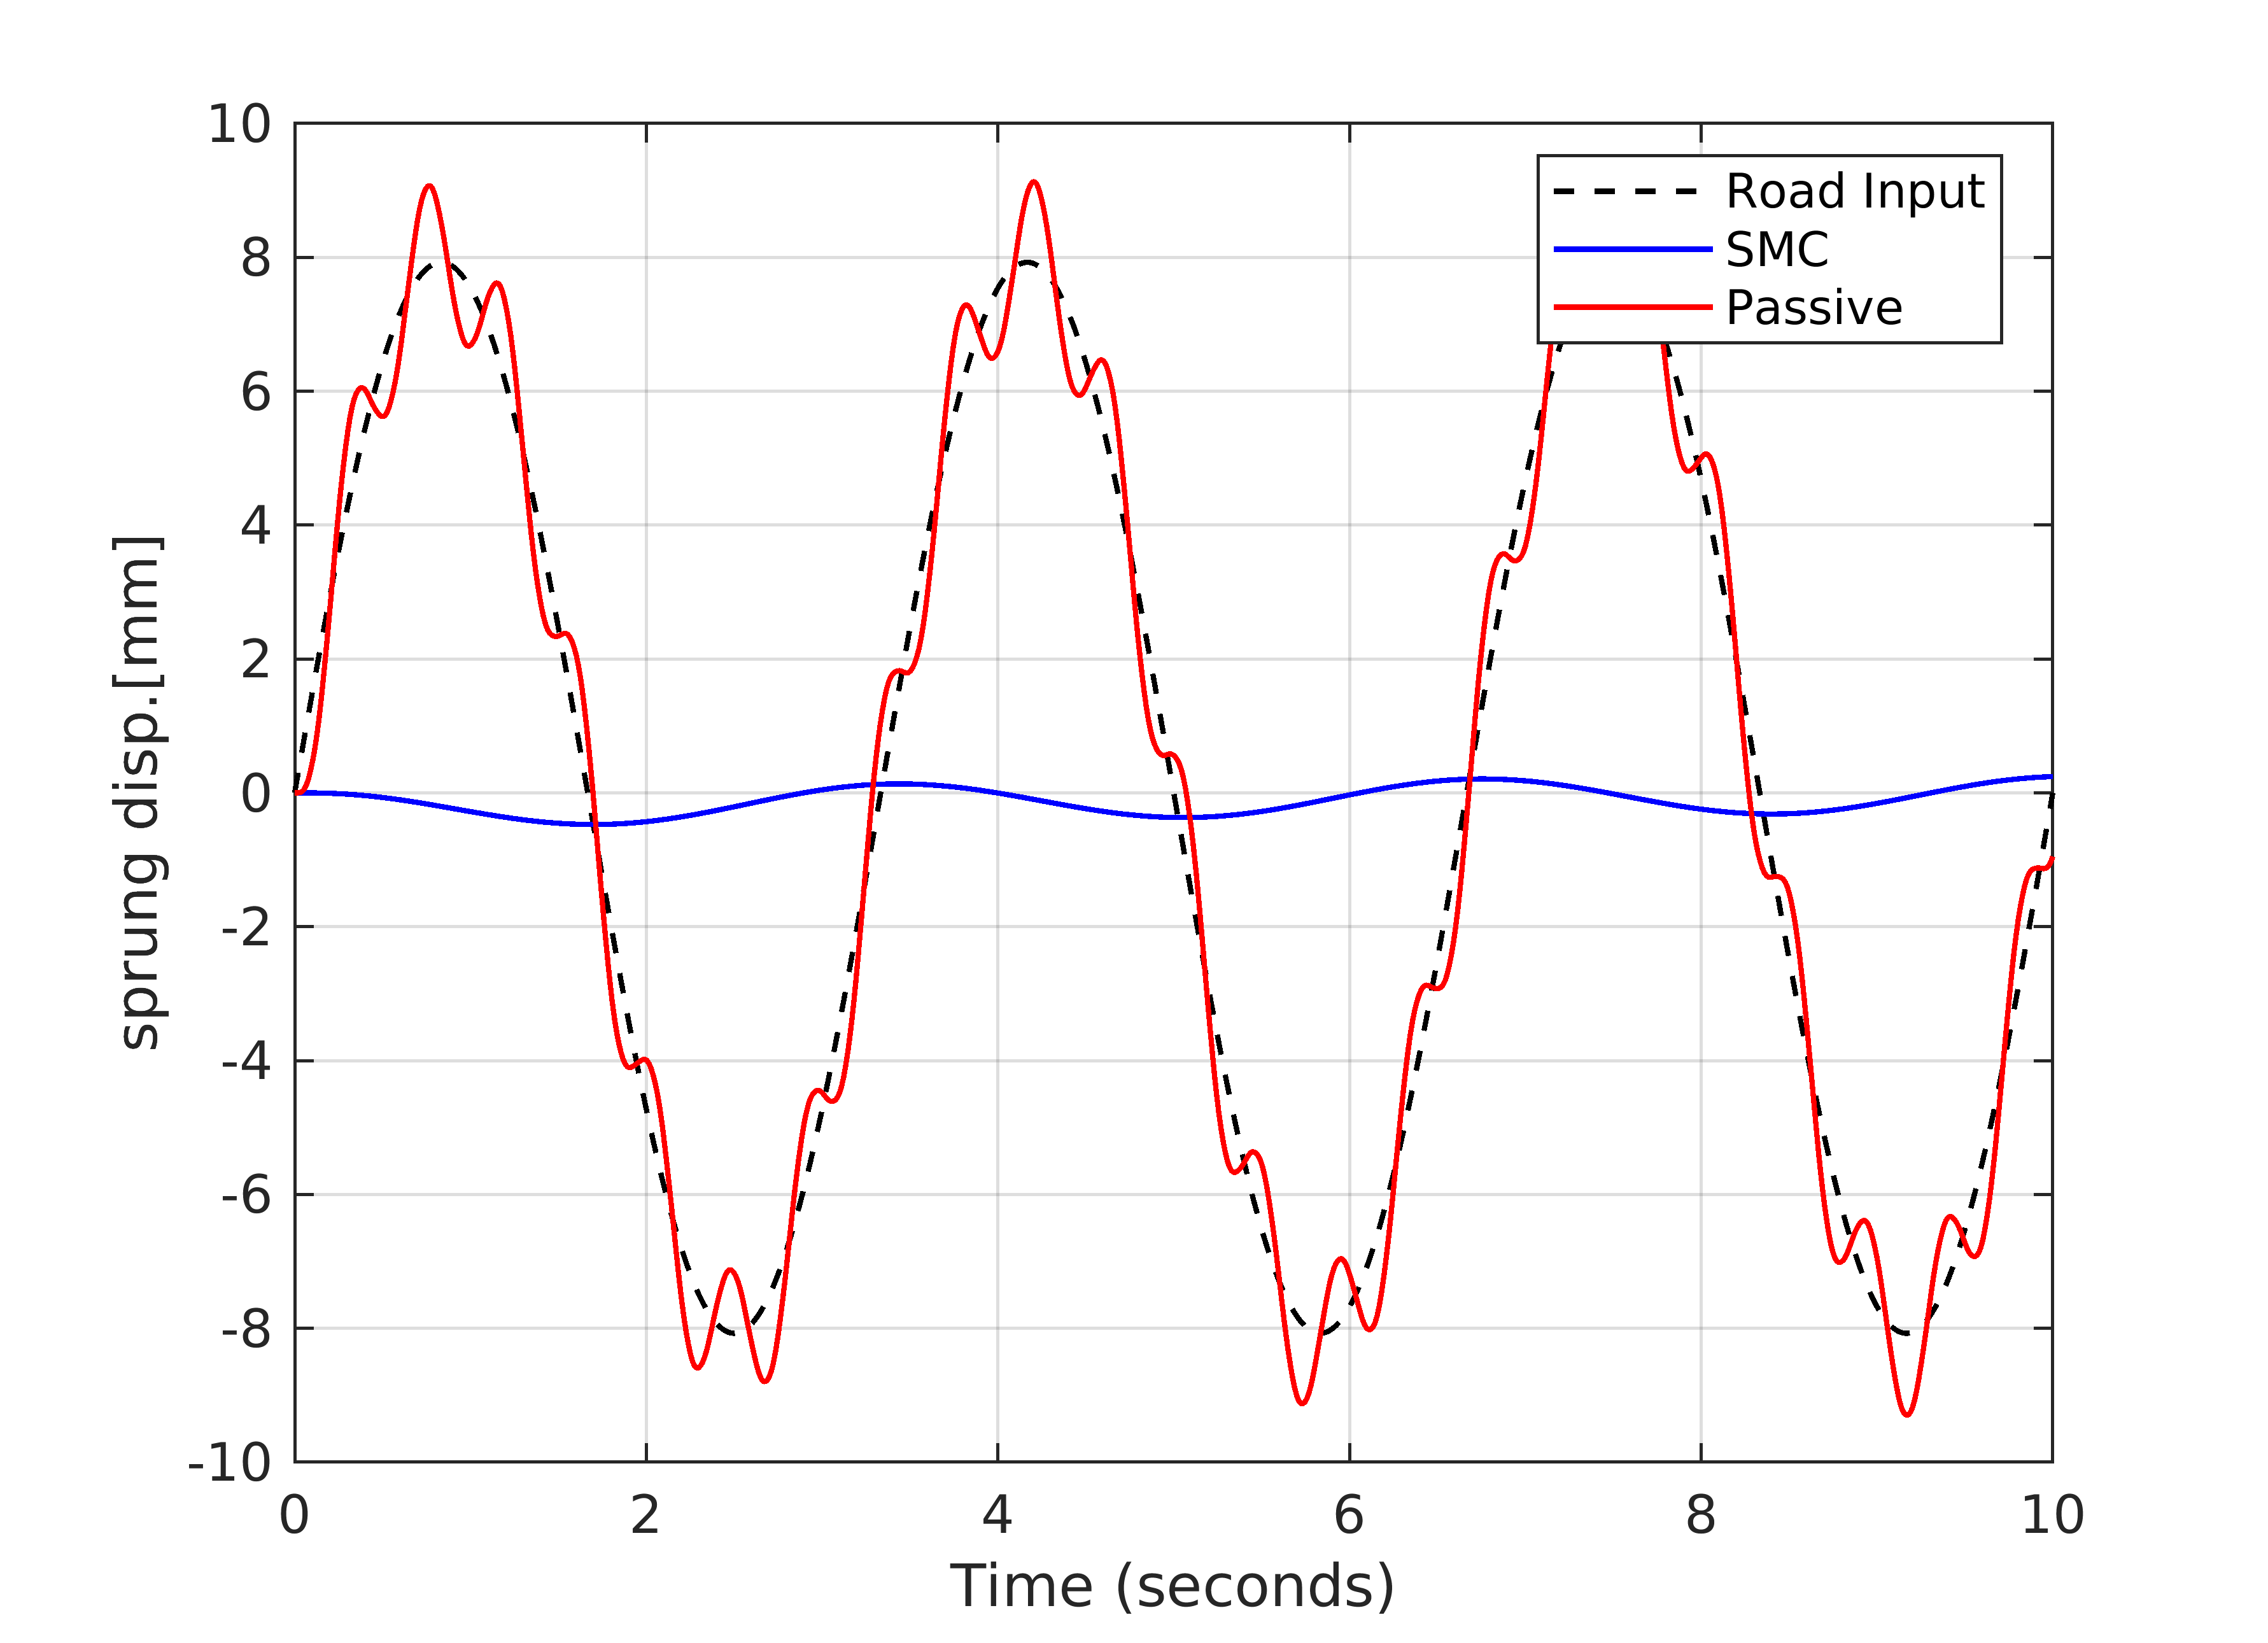
\includegraphics[trim=0cm 3cm 0cm 2cm, clip, width=0.6\textwidth]{SD}
	\caption{Sprung mass displacement. }
\end{figure}

\begin{figure}[H]
	\centering
	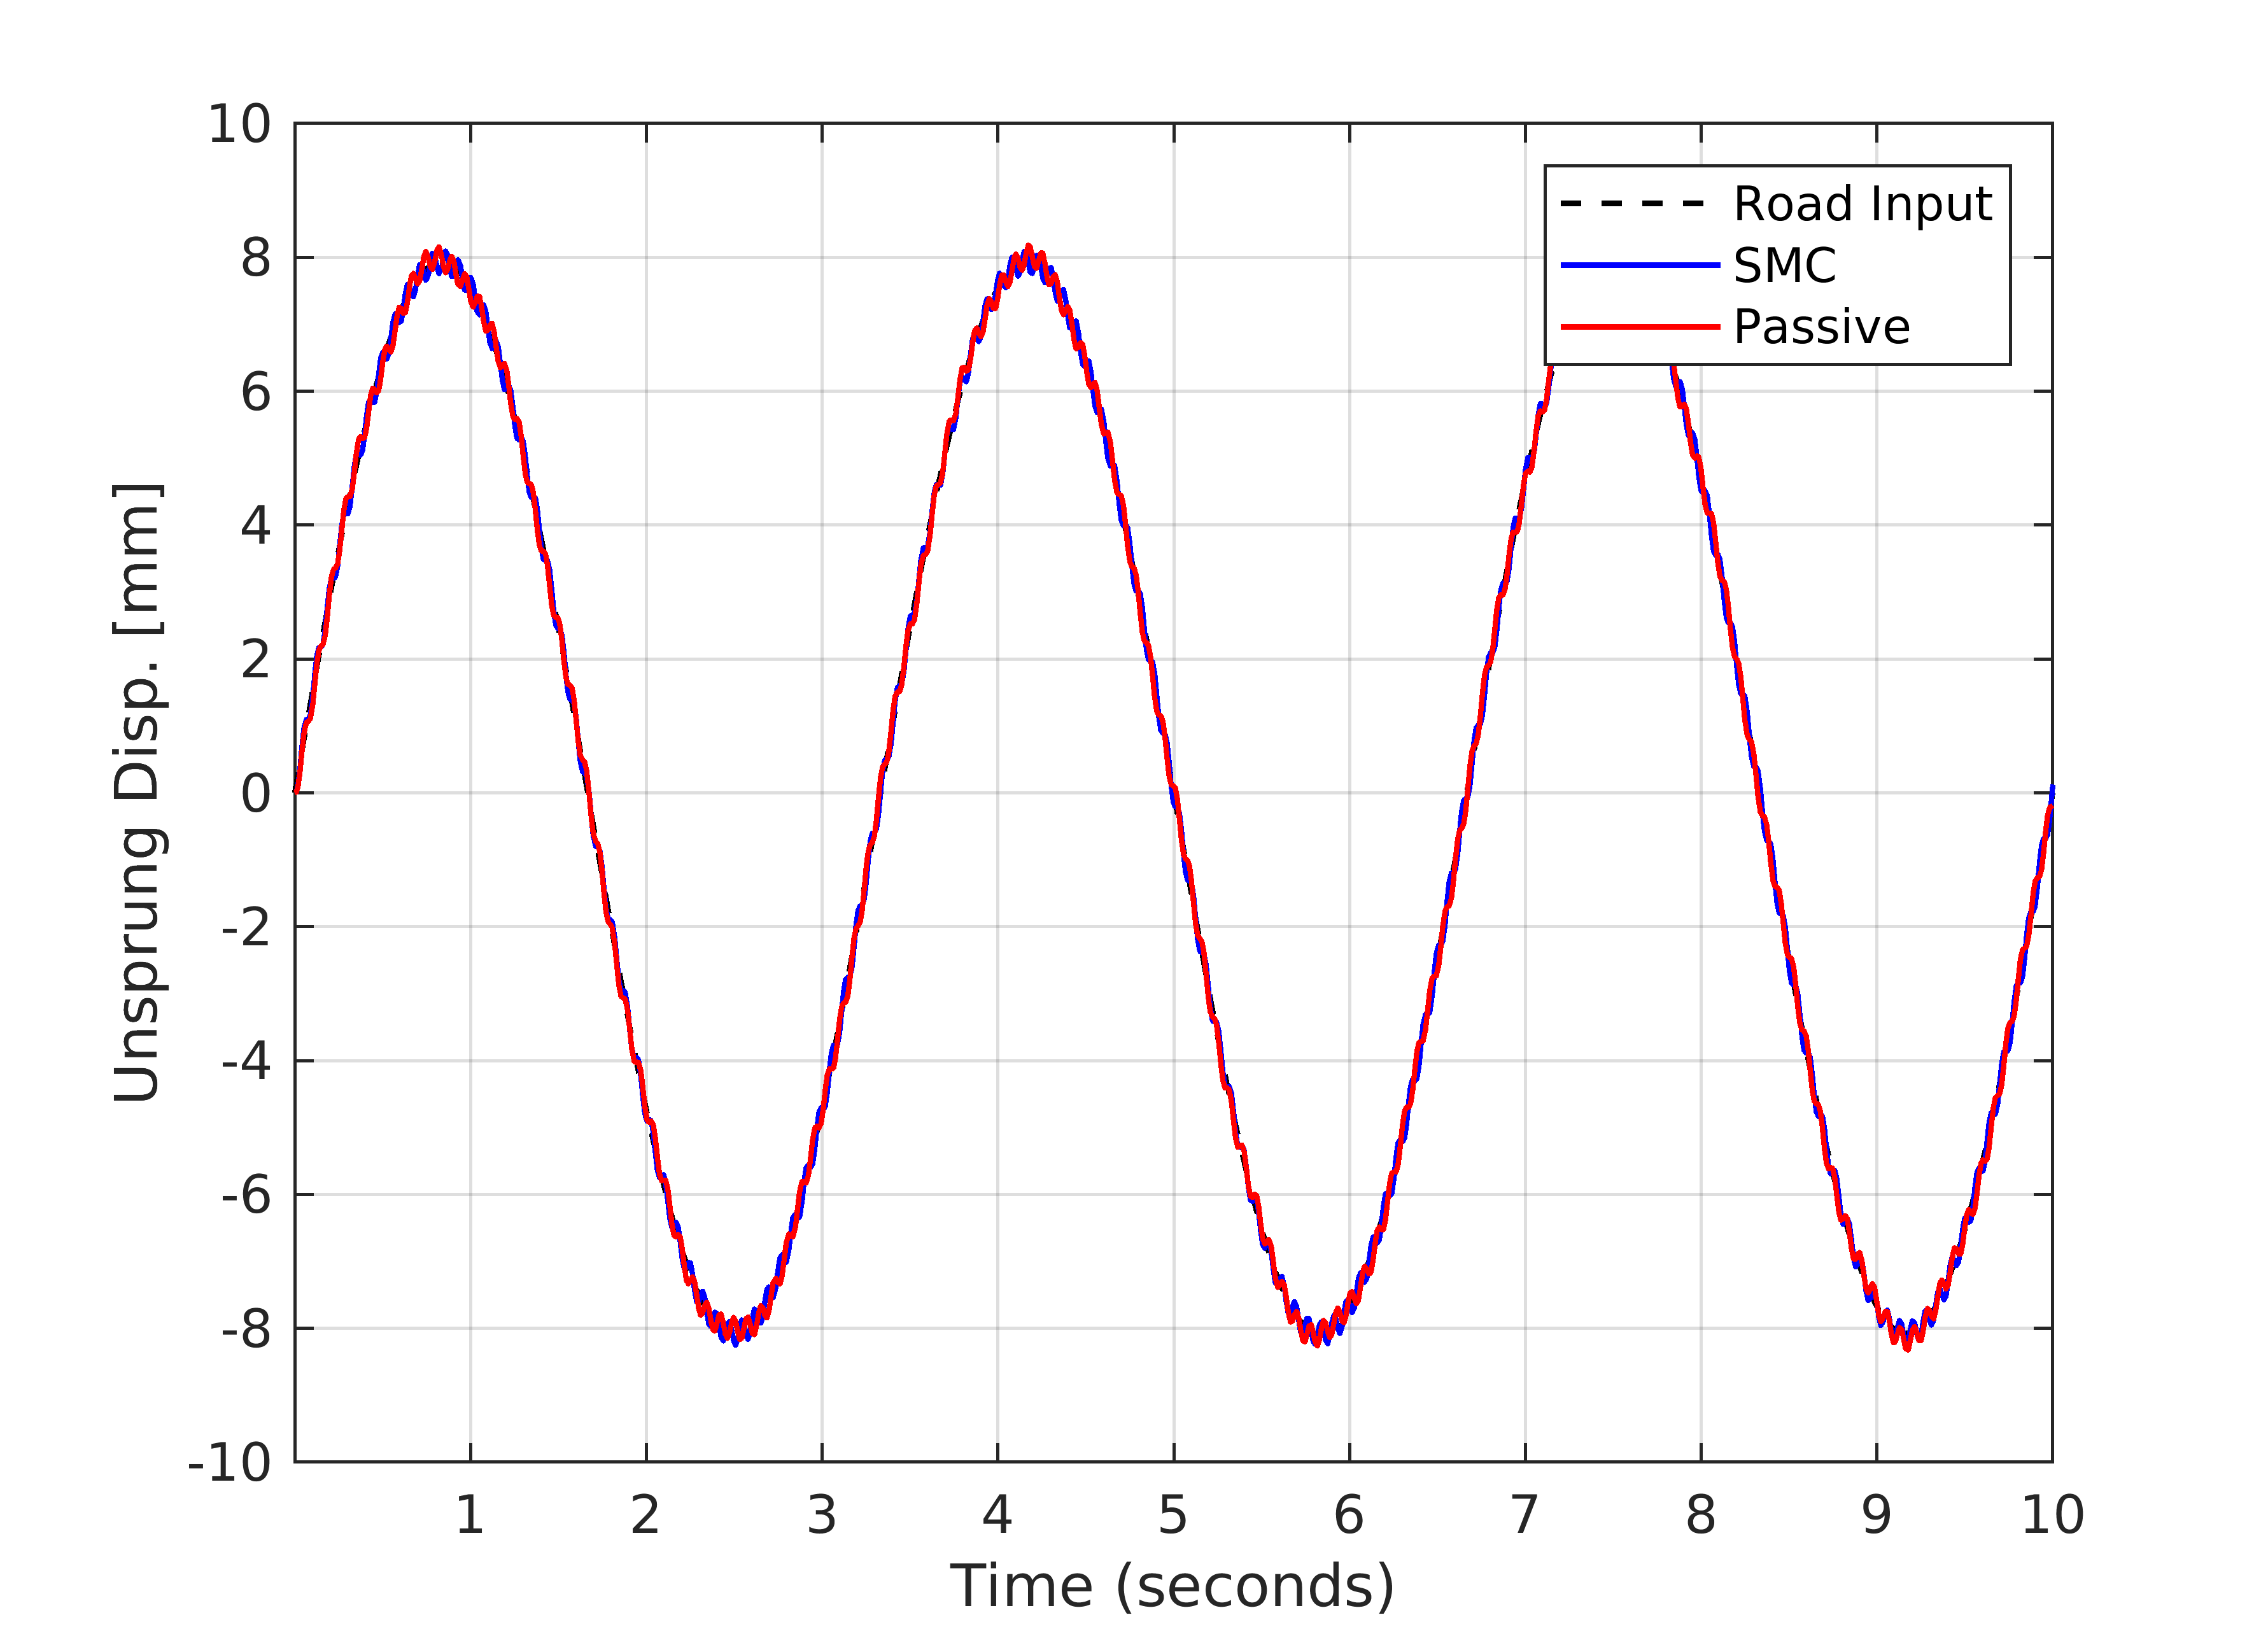
\includegraphics[trim=0cm 3cm 0cm 2cm, clip, width=0.6\textwidth]{usd}
	\caption{Usprung mass displacement. }
\end{figure}

\begin{figure}[H]
	\centering
	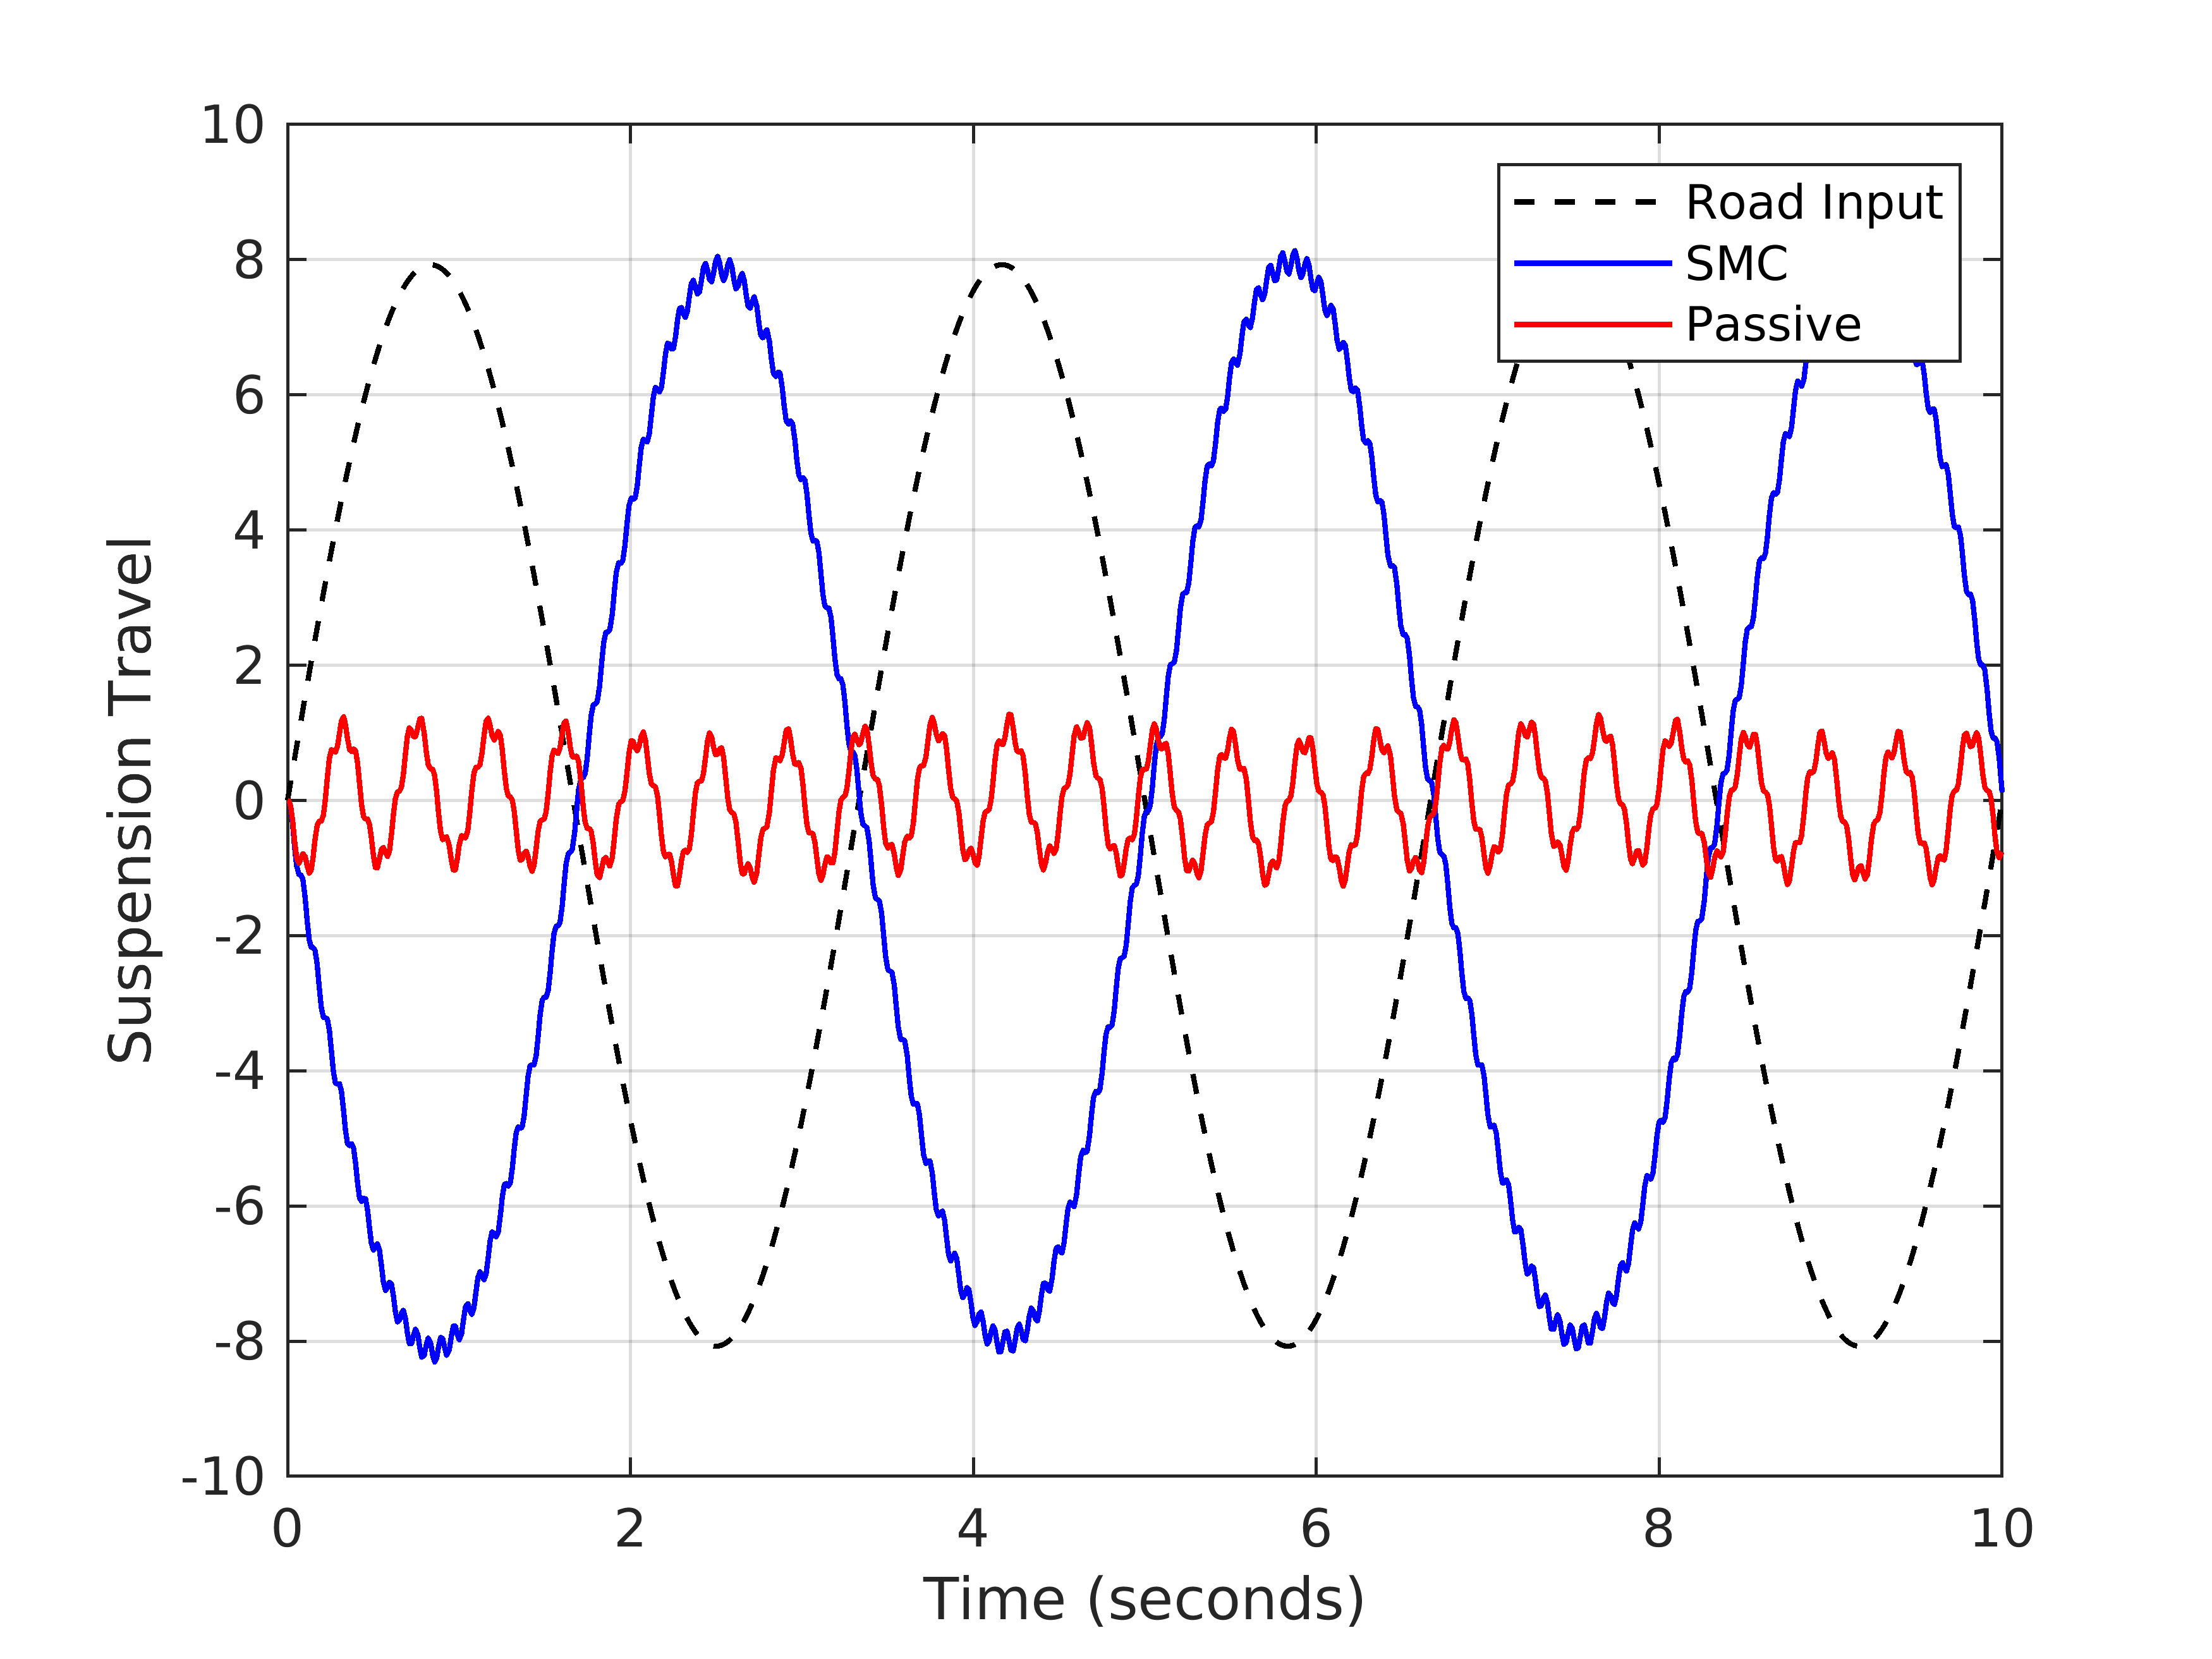
\includegraphics[trim=0cm 3cm 0cm 2cm, clip, width=0.6\textwidth]{sus t}
	\caption{Suspension travel. }
\end{figure}

\begin{figure}[H]
	\centering
	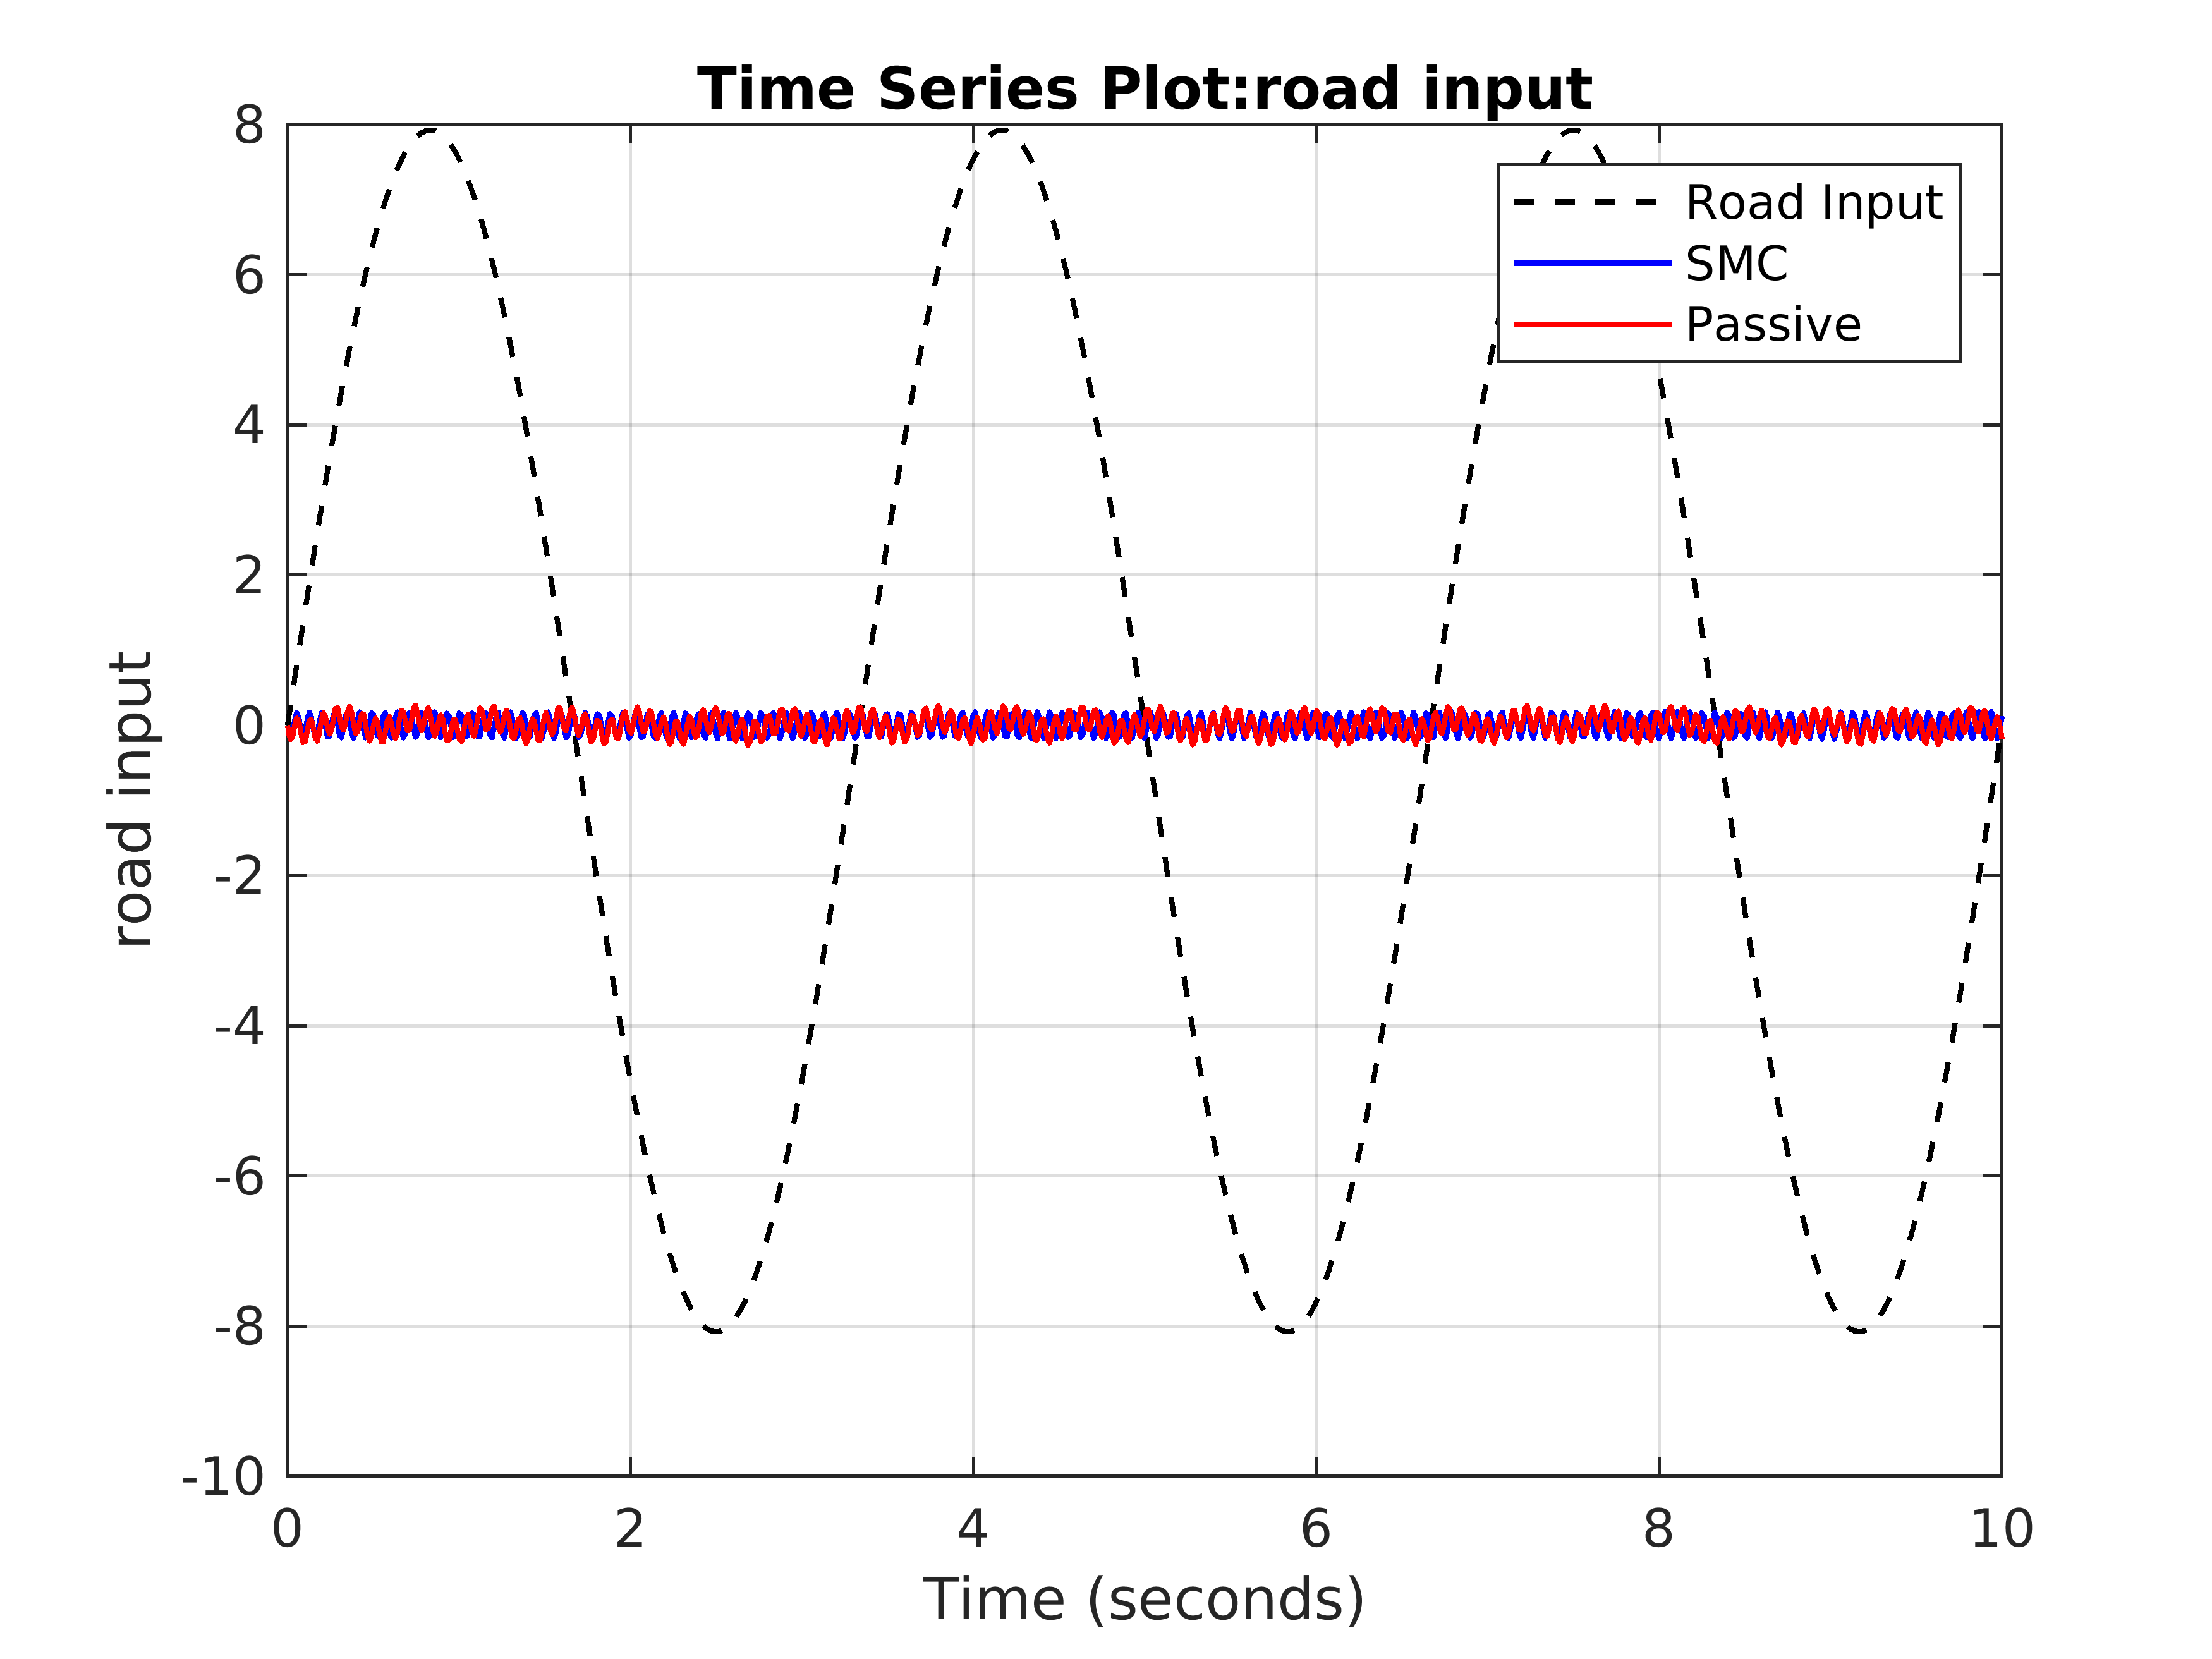
\includegraphics[trim=0cm 3cm 0cm 2cm, clip, width=0.6\textwidth]{TD}
	\caption{Dynamic tire defeliction. }
\end{figure}

\begin{figure}[H]
	\centering
	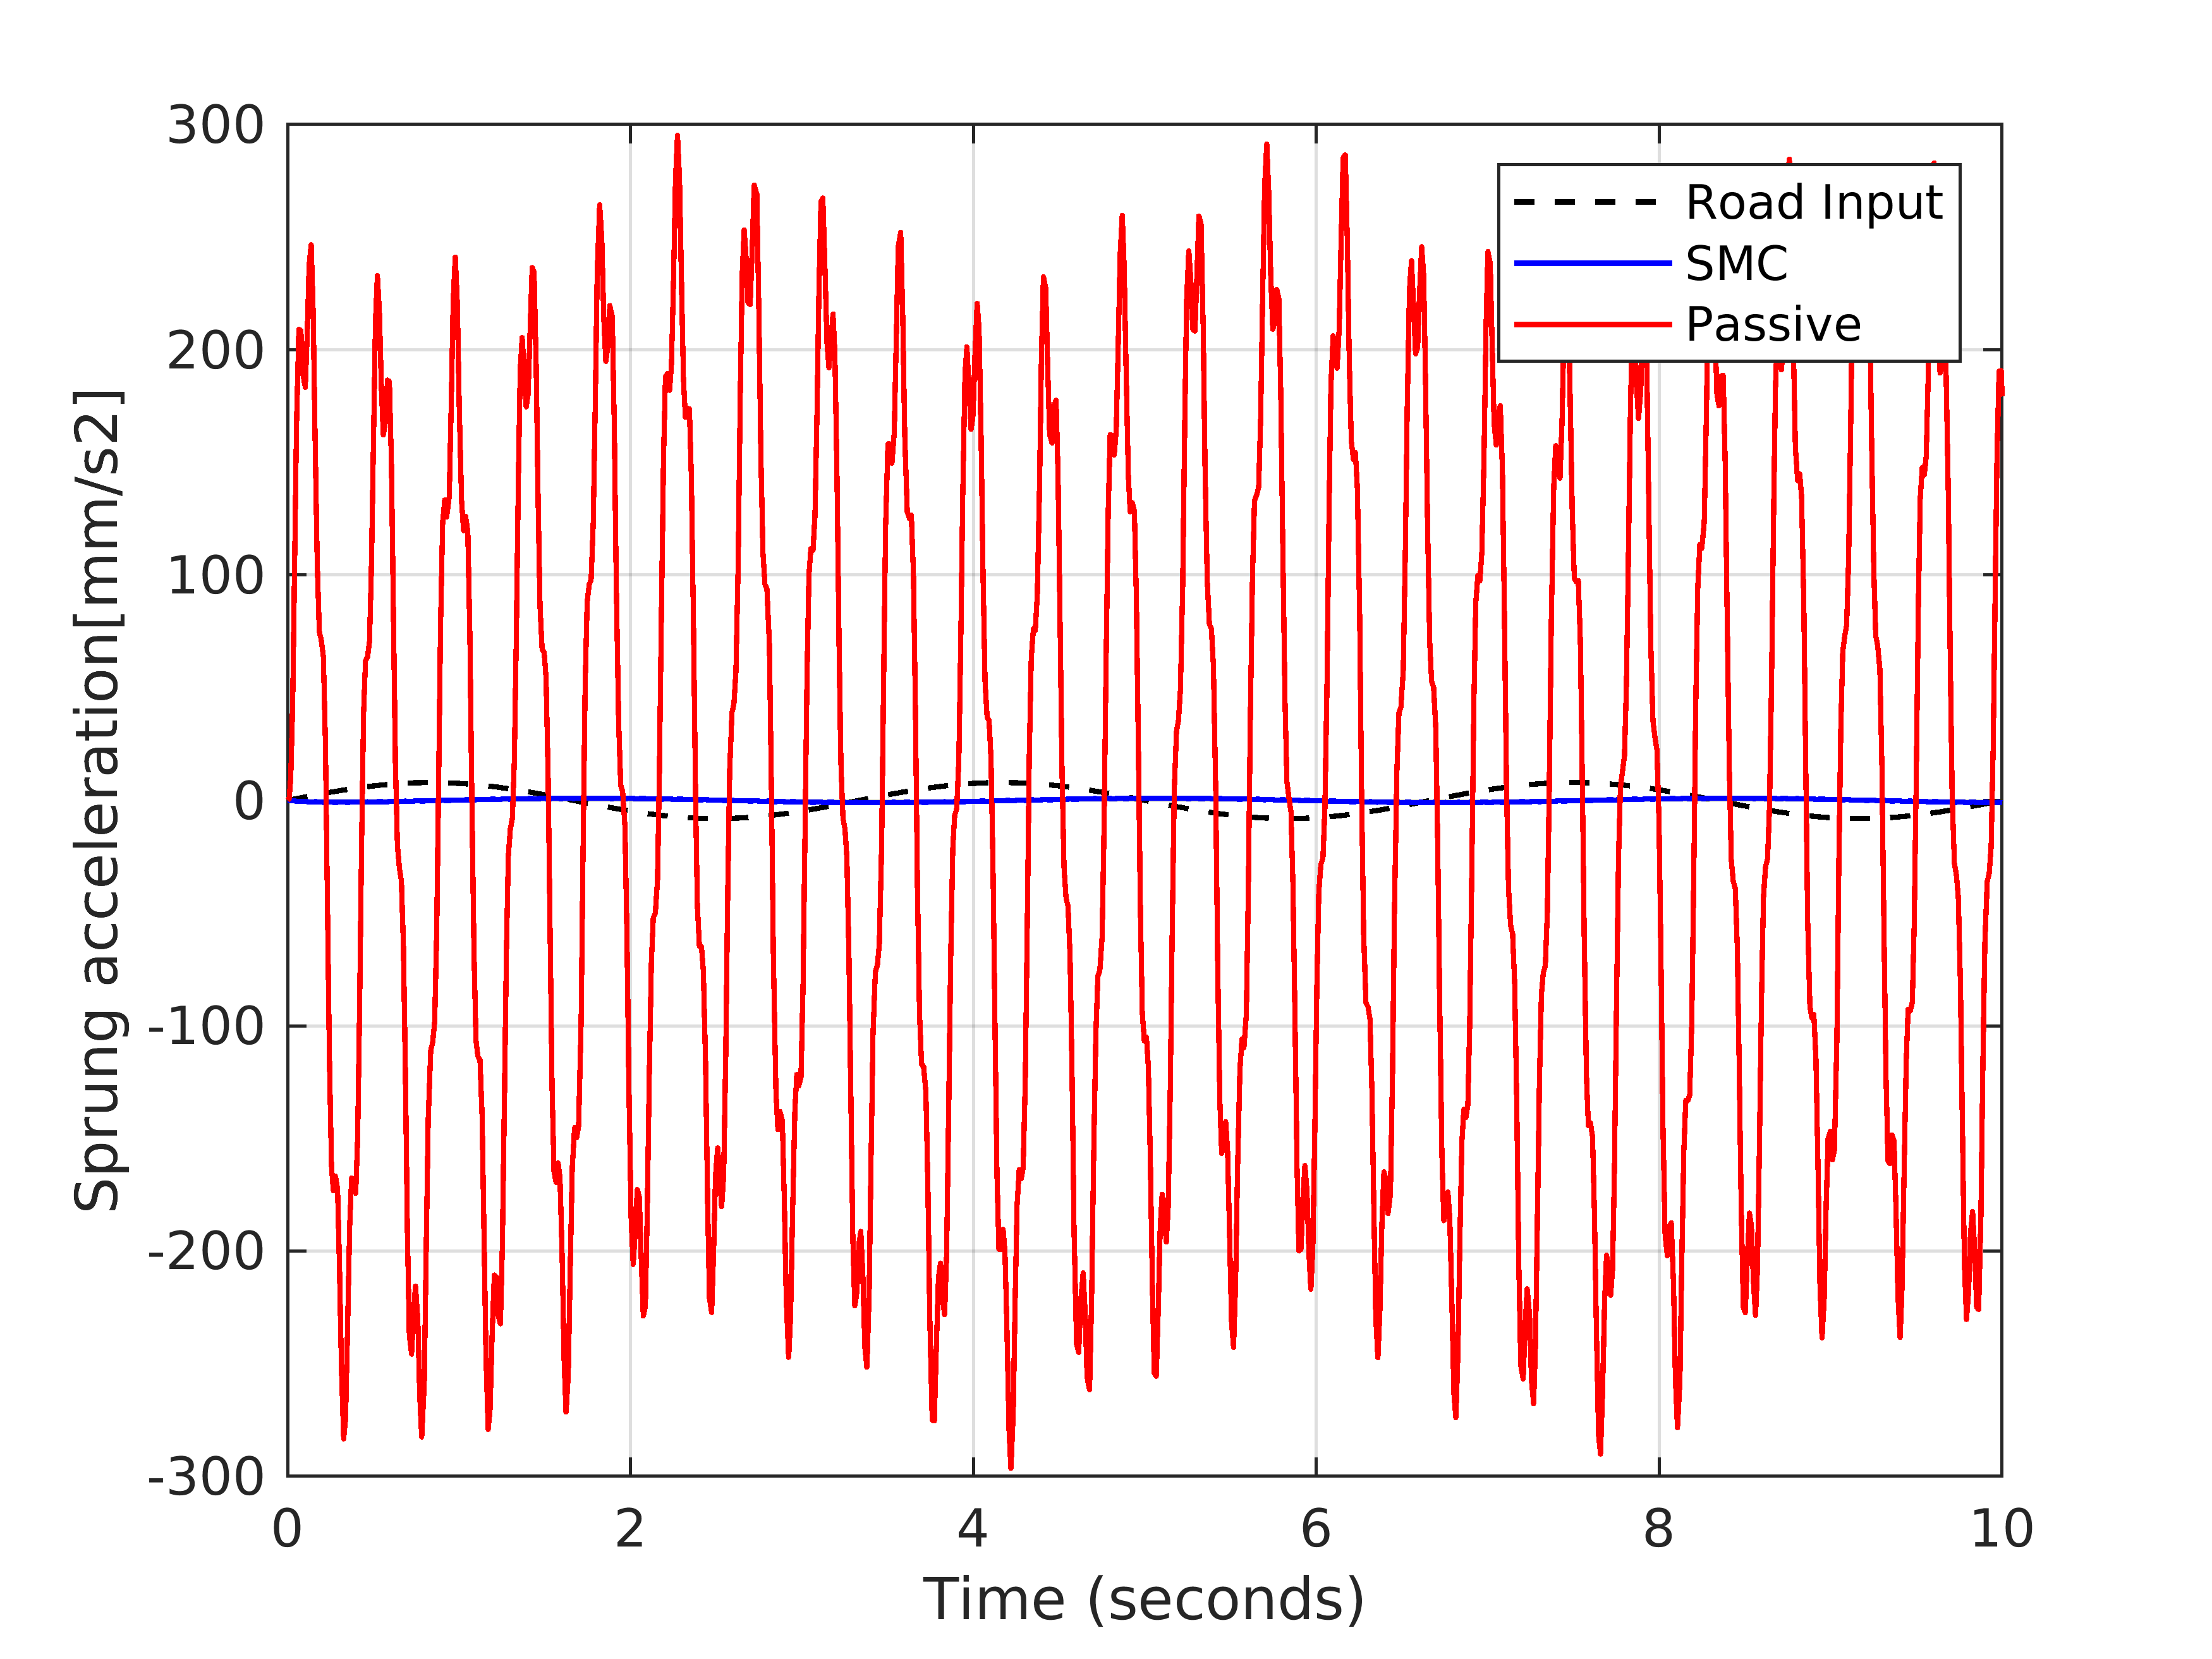
\includegraphics[trim=0cm 3cm 0cm 2cm, clip, width=0.6\textwidth]{accel}
	\caption{Sprung mass acceleration. }
\end{figure}

\begin{figure}[H]
	\centering
	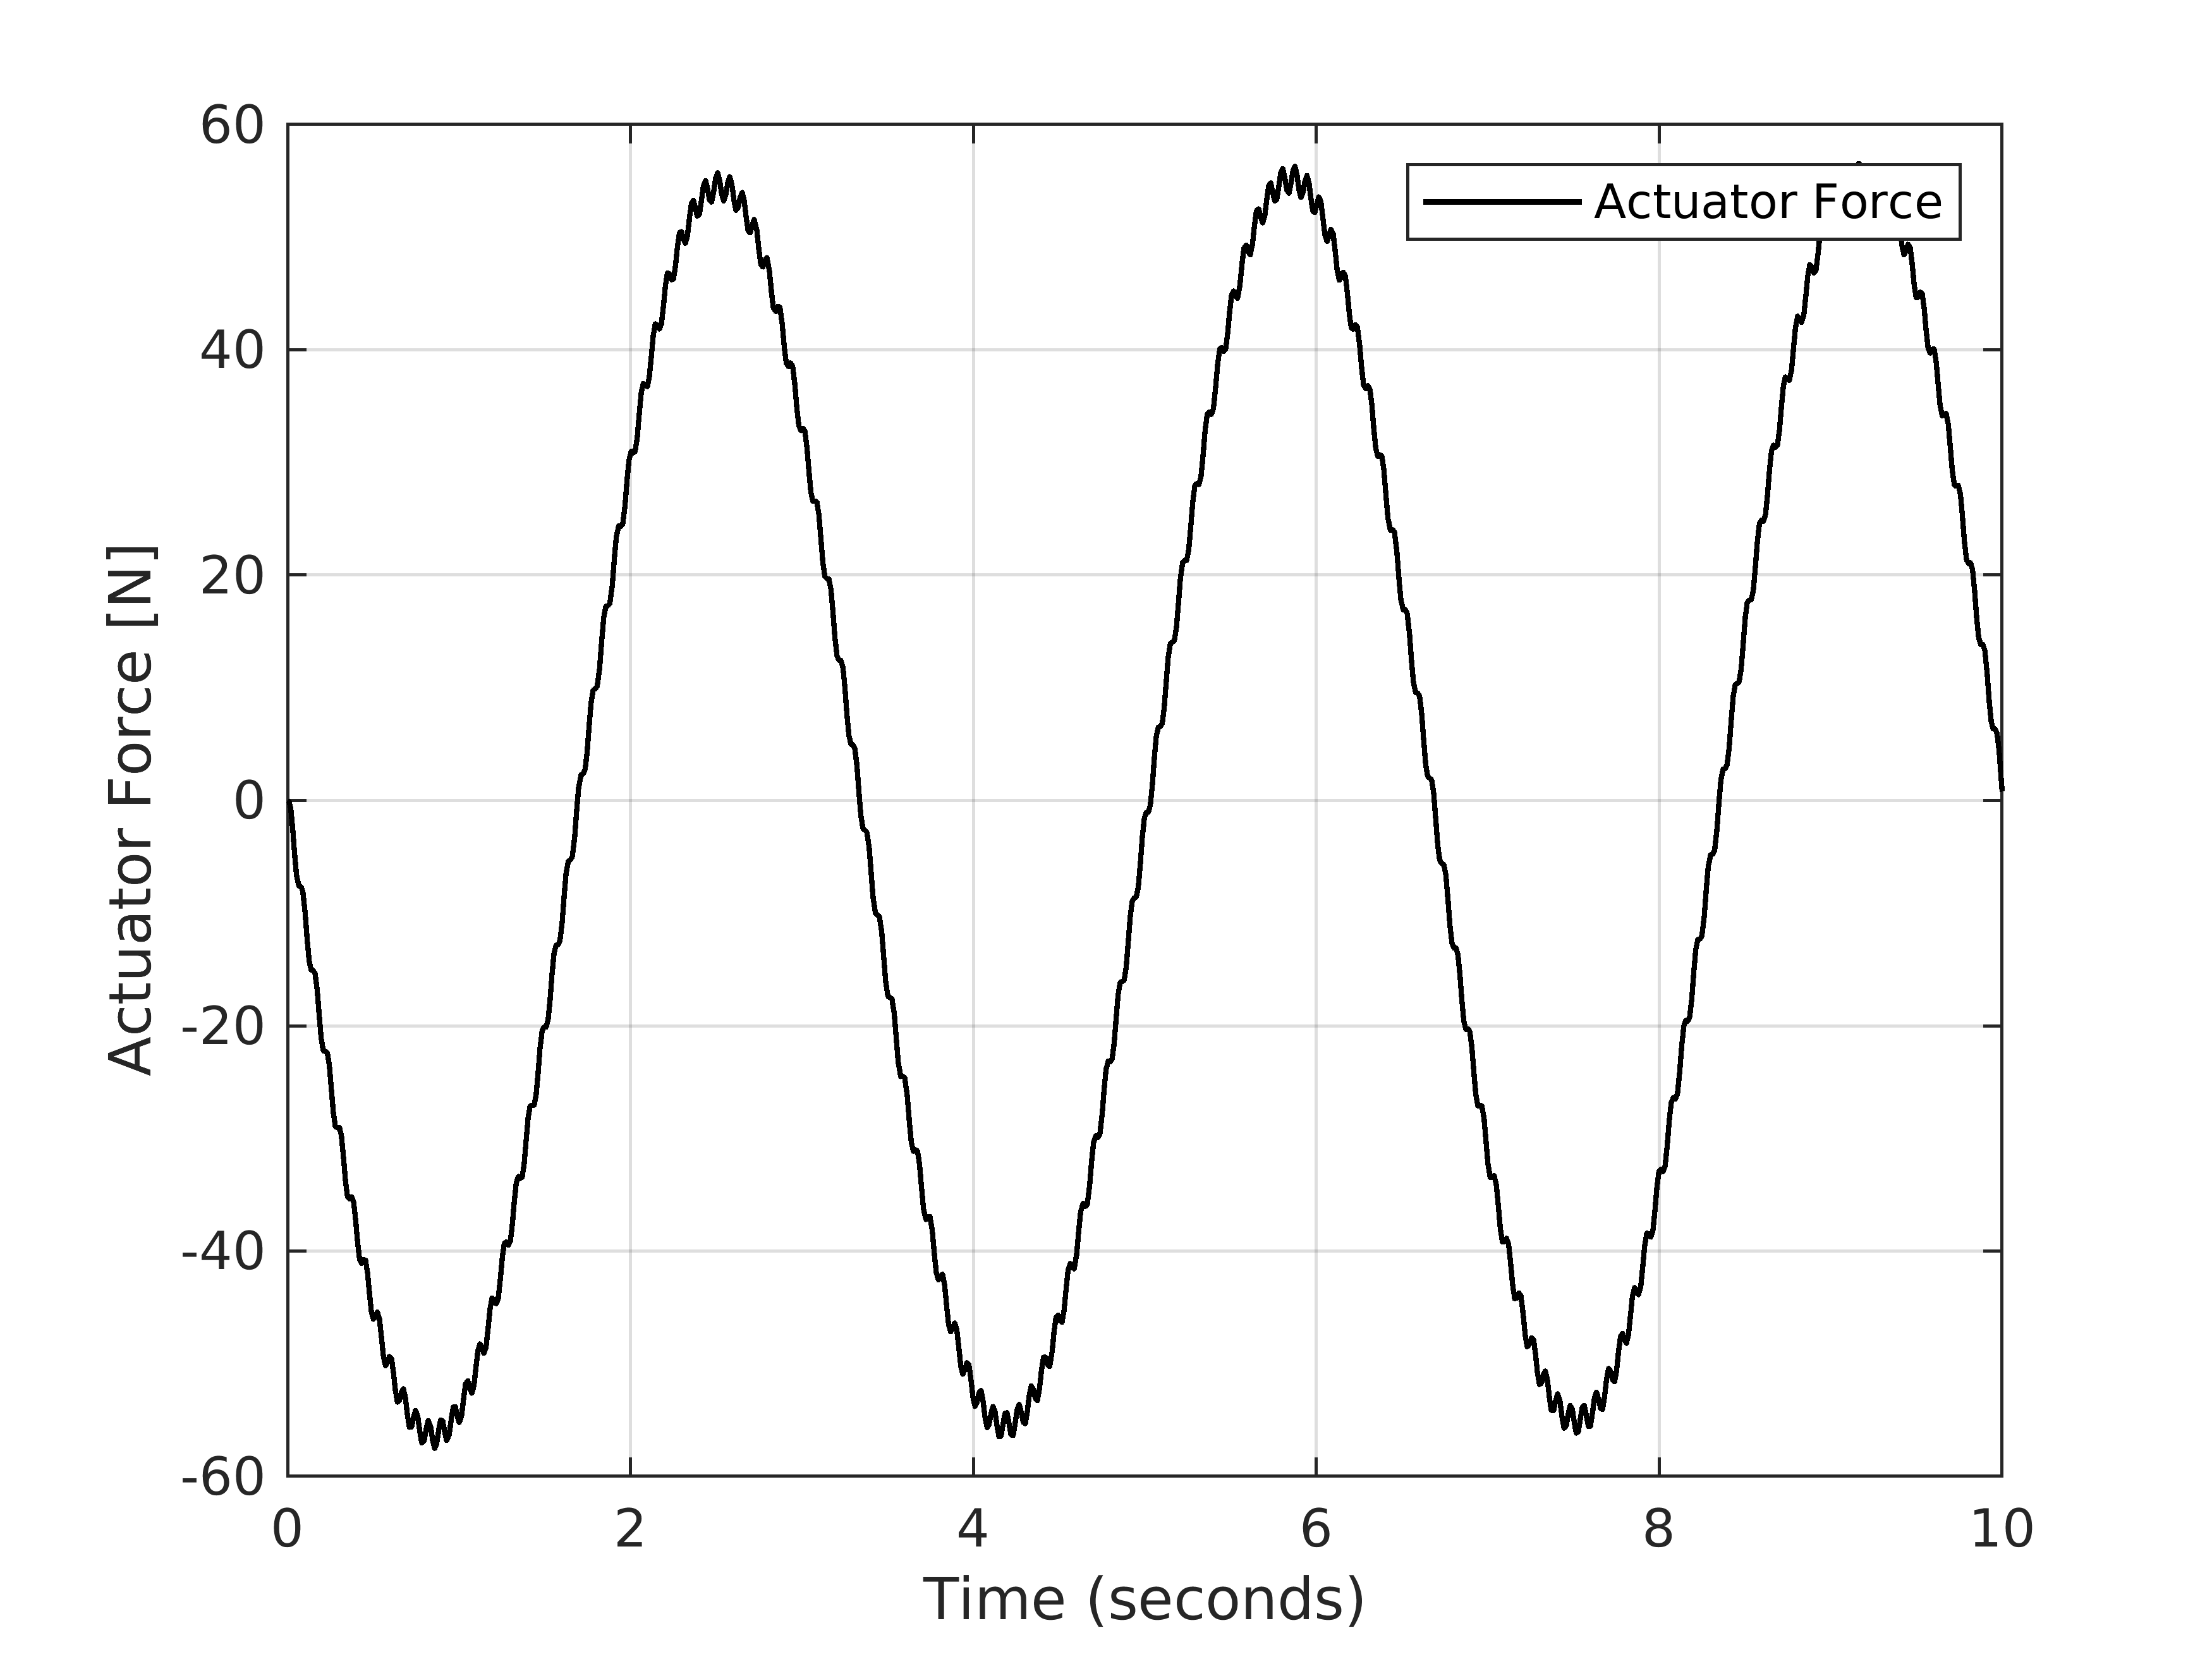
\includegraphics[trim=0cm 3cm 0cm 2cm, clip, width=0.6\textwidth]{force}
	\caption{Force. }
\end{figure}

